\documentclass[a4paper,11pt]{article}
\usepackage{jheppub} % for details on the use of the package, please see the JINST-author-manual
\usepackage{lineno}
\usepackage{xspace}
%\linenumbers

\usepackage[normalem]{ulem}
\usepackage{xcolor}
\newcommand{\del}[1]{\textcolor{red}{\sout{#1}}}
\newcommand{\add}[1]{\textcolor{blue}{#1}}
\newcommand{\mgamcnlo}{MadGraph5\_aMC@NLO}

\newcommand{\lhuc}{LH\ensuremath{\mu}C\xspace}
\newcommand{\lhmuc}{LH\ensuremath{\mu}C\xspace}
\arxivnumber{1234.56789} % if you have one

\title{\boldmath White Paper on High Energy, High Luminosity Lepton-Hadron Colliders at CERN}

\collaboration{(HELP4CERN Collaboration)}


%% [A] If main author
\collaboration{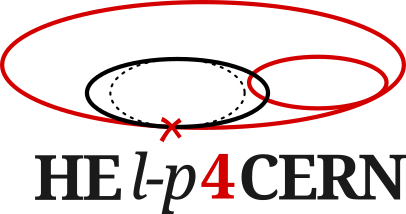
\includegraphics[height=17mm]{help4cern_logo_v1.png}\\
\vspace{2mm}}

%% or
%% [B] If "on behalf of"
%% \collaboration[c]{on behalf of XXX collaboration}


% Authors
% The "\note" macro will give a warning: "Ignoring empty anchor...", you can safely ignore it.

%% [A] simple case: 2 authors, same institution
%% \author[1]{A. Uthor\note{Corresponding author.}}
%% \author{and A. Nother Author}
%% \affiliation{Institution,\\Address, Country}

%% or, e.g.
%% [B] more complex case: 4 authors, 3 institutions, 2 footnotes
%% \author[a,b]{F. Irst,\note{Now at another university}}
%% \author[c]{S. Econd,}
%% \author[a,2]{T. Hird\note{Also at Some University.}}
%% \author[c,2]{and Fourth}
%% \affiliation[a]{Institution_1,\\Address, Country}
%% \affiliation[b]{Institution_2,\\Address, Country}
%% \affiliation[c]{Institution_3,\\Address, Country}
\author[a]{D.~Acosta,}
\affiliation[a]{Rice U.}

\author[b]{D.~Britzger,}
\affiliation[b]{Max-Planck-Institut f\"ur Physik, Boltzmannstr. 8, 85748 Garching, Germany}

\author[c]{A.C.~Canbay,}
\affiliation[c]{Department of Physic, Ankara University, Ankara 06100, Turkiye}

\author[def]{K.~Cheung,}
\affiliation[d]{Department of Physics, National Tsing Hua University, Hsinchu 300, Taiwan}
\affiliation[e]{Center for Theory and Computation, National Tsing Hua University, Hsinchu 300, Taiwan}
\affiliation[f]{Department of Physics, Konkuk University, Seoul 05029, Republic of Korea}

\author[g]{B.~Dagli,}
\affiliation[g]{TOBB University of Economics and Technology, Ankara 06560, Turkiye}

\author[h]{L.~Forthomme,}
\affiliation[h]{AGH University of Krakow, Faculty of Physics and Applied Computer Science, Al. Mickiewicza 30, 30-055 Kraków, Poland}

\author[i]{B.~Holzer,}
\affiliation[i]{CERN, Meyrin, Switzerland}

\author[j]{U.~Kaya,}
\affiliation[j]{Institute of Accelerator Technologies Ankara University, Ankara 06830, Turkiye}

\author[h]{H.~Khanpour,}

\author[k]{A.~Kilic,}
\affiliation[k]{Department of Physics, Bursa Uludağ University, 16210 Bursa, Turkiye}

\author[k]{F.~Kocak,}

\author[h]{P.~Kotko,}

\author[l]{M.~Kumar,}

\author[m]{K.~Long,}
\affiliation[m]{Imperial C.}

\author[n]{X.~Lu,}
\affiliation[n]{Warwick U.}

\author[l]{B.~Mellado,}
\affiliation[l]{School of Physics and Institute for Collider Particle Physics, University of the Witwatersrand, Wits, 2050, Johannesburg, South Africa}

\author[o]{S.~Moretti,}
\affiliation[o]{University of Southampton, School of Physics and Astronomy, Southampton SO17 1BJ, UK \&\\
Department of Physics and Astronomy, Uppsala University, Box 516, SE-751 20 Uppsala, Sweden}

\author[p]{M.~Otani,}
\affiliation[p]{KEK}

\author[h]{K.~Piotrzkowski,}

\author[q]{C.~Rogers,}
\affiliation[q]{RAL}

\author[i]{D.~Schulte,}

\author[r]{A.M.~Sta\'sto,}
\affiliation[r]{Department of Physics, Penn State University, University Park, PA 16802, U.S.A.}

\author[g]{S.~Sultansoy,}

\author[k]{I.~Tapan,}


\author[s]{S.~Tentori,}
\affiliation[s]{Center for Cosmology, Particle Physics and Phenomenology, Universit\'e catholique de Louvain, Louvain-la-Neuve, Belgium}

\author[t]{M.~Topp-Mugglestone,}
\affiliation[t]{Oxford U.}

\author[u]{Z.S.~Wang,}
\affiliation[u]{School of Physics, Hefei University of Technology, Hefei 230601, People’s Republic of China}

\author[v]{Y. Yamazaki,}
\affiliation[v]{Kobe U.}

\author[w]{C.~Zhang,}
\affiliation[w]{Liverpool U.}

\author[h]{G.~Ziarko,}

\author[i]{F.~Zimmermann}
%\author{\\ The HELP4CERN Study Group}
%\affiliation{One University,\\some-street, Country}

% E-mail addresses: only for the corresponding author
%\emailAdd{first@one.univ}
\emailAdd{help-4-cern@cern.ch}

\abstract{
\vspace{6mm}\\
The main objective of this white paper is to present to the HEP community the latest developments in high energy, high luminosity lepton-hadron colliders, which were triggered by a recent proposal to perform muon-hadron collisions at the HL-LHC~\cite{Akturk:2025ubm}, using the infrastructure of the energy recovery linac (ERL) proposed for the electron-hadron collider LHeC~\cite{LHeCStudyGroup:2012zhm,LHeC:2020van,Ahmadova:2025vzd}.

In the following it is assumed that nominally the \lhuc will deliver collisions of 1~TeV muons with 7 TeV protons at the HL-LHC, corresponding to $\sqrt{s_{\mu p}}=5.3$~TeV, therefore much higher than the $ep$ centre-of-mass energy at the proposed FCC-eh. The expected \lhuc peak luminosity is about $10^{34}$cm$^{-2}$s$^{-1}$, making it effectively a Higgs-Electroweak-Top (HET) factory. Moreover, an option of 2 TeV muon beam is also considered, resulting in the centre-of-mass energy $\sqrt{s_{\mu p}}= 7.5$~TeV. For the physics cases discussed below, the following ultimate integrated luminosities are assumed:
1~ab$^{-1}$ for the LHeC and \lhuc, and in addition
250~fb$^{-1}$ for the 1 TeV case of \lhuc.

Already an initial running of the \lhuc at very low luminosity will allow a huge expansion in the $(x, Q^2)$ plane: by an order of magnitude with respect to the LHeC and by more than two orders wrt. HERA.
As a result, unique studies of parton non-linear effects at the LHeC can be further extended, including  powerful insights into evasive nuclear effects in the muon-ion scattering. In addition, PDF flavor decomposition can also be further improved, as well as precision measurements of $\alpha_S$, which are of high relevance for research at the HL-LHC and future hadron colliders.

In the Higgs boson sector, the \lhuc offers similar of even better sensitivity to the Higgs couplings than the LHeC, see Table~\ref{tab:i} below, hence many significant improvements are expected with respect to the Higgs boson prospects at the HL-LHC alone. Particularly valuable will be the \lhuc contributions to the Higgs couplings to Z and W bosons, which will be highly relevant even during the FCC-ee era~\cite{Ahmadova:2025vzd,Cheung:2021iev}.

In the context of determination of the electroweak parameters, \lhuc also offers improvements over the LHeC~\cite{Ahmadova:2025vzd} by precision measurements of $M_W$ and $\sin^2{\theta_W}$, due to significantly larger span in $Q^2$.

In addition, the LH$\mu$C will be a real top quark factory, particularly well suited for precision studies near the production threshold, and including precise measurements of the top charge. Moreover, similarly to the LHeC, it is expected to make unique contributions to studies of single top production and of rare top decays~\cite{Ahmadova:2025vzd}.  

Last but not least, due to its high centre-of-mass energy and unique initial state, the \lhuc will serve also as a very significant platform for the BSM searches~\cite{Cheung:2021iev}.

In this white paper, the concepts of all components of the proposed \lhuc facility are presented:
From ultra-cold $\mu^+$-source and $\mu^+$ booster, through the $\mu^+$ main ring, to the interaction region and machine-detector interface (MDI). This includes discussions of alternative scenarios and possible optimisations,
including operation of the proton ring at the \lhuc.

Moreover, not only a comprehensive overview of the developments of high energy-lepton colliders is presented, but also a concrete proposal for an action plan, in particular in relation to further developments of the \lhuc concept:
\begin{itemize}
    \item in-depth Monte Carlo studies of the ultra-cold $\mu^+$-source ;
    \item full simulation studies of the vFFA beam dynamics including ERL ;
    \item first conceptual proposals for the beam separation scheme and MDI ;
    \item calculations of the beam-beam effects and the luminosity optimisation ;
    \item scenarios for the 2 TeV upgrade options.
\end{itemize}

Finally, it should be stressed that the \lhuc project on the one hand profusely benefits from the developments within the Muon Collider project and of ultra-cold muon beams in general, but on the other hand it would constitute a very major stepping stone in further R\&D developments for these projects. In addition, the \lhuc project very much strengthens the case for the LHeC and much intensified work towards its realisation. Moreover, the \lhuc project creates an exciting possibility of a platform for new research in neutrino physics at CERN, and elsewhere, including also the science made with novel ultra-cold intense muon sources.  Last but not least, the \lhuc project opens an amazing opportunity to largely extend the science programme at the proposed FCC-hh (HE-LHC) facility by adding, at a fractional cost, a very powerful muon-hadron collider, capable of colliding muons and protons at 30(15)~TeV! And of producing very high flux neutrino beams for research. 

\paragraph{
[it is a temporary version having form of "executive summary"]\\}
}


\begin{document}
\maketitle
\flushbottom

\section{Introduction}
\label{sec:intro}

[Krzysztof, Saleh]\\


LHeC~\cite{LHeC:2020van,Ahmadova:2025vzd}, Stage one~\cite{Andre:2025iar}, LHeC@IP2~\cite{Andre:2022xeh}
\lhuc~\cite{Akturk:2025ubm}, $\mu$TRISTAN~\cite{Hamada:2022mua}, ultra cold $\mu$~beam~\cite{Aritome:2024rlu}

\newpage

\section{Physics case}
\label{sec:physics}

[Ali Can, Hamzeh]\\

The comprehensive overview of $eh$ physics is available in the LHeC CDR~\cite{LHeC:2020van}, with many relevant updates given in the recent LHeC ESPP paper~\cite{Ahmadova:2025vzd}. Some supplementary information is given in the 20 GeV LHeC proposal~\cite{Andre:2025iar}. A very useful discussion of part of $\mu p$ physics is available in Ref.~\cite{Cheung:2021iev}.
\vspace{4mm}

\add{FIXME: to be updated from 50 GeV to 60 GeV!!}

\begin{table}[htbp]
\centering
\begin{tabular}{c||c|c|c|c|c}
\hline
Process & {\small20\,GeV\,LHeC} & {\small 60\,GeV\,LHeC} & {\small 500\,GeV\,\lhuc} & {\small 1\,TeV\,\lhuc} & {\small 2\,TeV\,\lhuc} \\
\hline
$\sigma$($l\,p\to \nu_l \,H~{\rm +~jet}+X$) [pb] &  0.052 & 0.197 & 0.656 (unpol. 0.438) & 1.092 & 1.744\\
$\sigma$($l\,p\to l\,H~{\rm +~jet}+X$) [pb] & 0.0056 & 0.024 & 0.150(unpol. 0.135) & 0.245 & 0.383\\
$\sigma$($l\,p\to l\,t\bar{t}~+$~X) [pb] &  \add{0.0015} &  \add{0.0323} & \add{1.03} & \add{2.23} & \\
$\sigma$($l\,p\to \nu_l \,t~+$~X) [pb] &  \add{0.55} &  \add{2.89} &  \add{21.26} & \add{36.77} &\\
\hline
\end{tabular}
\caption{Inclusive cross-sections for four major processes at the 20 and 60 GeV LHeC as well as 500 GeV and 1~TeV LH$\mu$C. In the LHeC cases an 80\% electron beam polarisation is assumed~\cite{Andre:2025iar} while for LH$\mu$C the polarisation for the anti-muon beam is assumed to be 50\% .}
\label{tab:i}
\end{table}

The production cross-sections in Table~\ref{tab:i} are used to make tentative evaluations of the \lhuc physics potential by properly re-scaling the results obtained within the comprehensive LHeC studies~\cite{LHeC:2020van,Ahmadova:2025vzd}.
For these results, \mgamcnlo~\cite{Alwall:2014hca} is used with a \del{CT10} (\add{NNPDF23}) \add{Simone: in LHeC the simulation were done using cteq6l1 PDF, if we want to rescale the LHeC results I think it is better to keep the same PDF set. Furthermore the Higgs coupling extraction was done with 1.3TeV center of mass energy, corresponding th an electron beam of 60 GeV.}modelling at next-to-leading order of the parton distribution functions (PDFs).\add{Simone: I fixed the 1 TeV numbers taking into account the polarisation, however the number we inserted are LO, why are we putting +X in the Higgs case? I removed it}
\add{Simone: I don't know how the top production has been simulated, I cannot reproduce the numbers, can we put explicitly the cuts and include polarizations in the 1 TEV case?}
%None of the Higgs nor the top quarks are decayed, and therefore no branching fraction is applied to these cross sections.
%The generator-level acceptance cuts assumed are the following:

%Inclusive leading-order (LO) cross sections are evaluated for single-top and top–antitop production at the LHeC with 20 and 50,GeV lepton beams and at the LH$\mu$C with 500,GeV and 1,TeV muon beams. For the LHeC configurations we assume an 80% electron-beam polarisation. The calculations are performed for the core LO hard processes, i.e. without an explicit additional jet at the matrix-element level, and with generation cuts switched off ($p_T^\ell$, $\eta_\ell$, $p_T^j$, $\eta_j$). A common five-flavour scheme (5FS) is used throughout. The quoted results correspond to fixed-order, parton-level totals and therefore do not depend on parton-shower or initial-state-radiation settings. We use LO matrix elements combined with NLO proton PDFs, adopting the MadGraph default set (NNPDF23).



One should stress that, as at the LHeC, in general the expected detector acceptances are high at the LH$\mu$C, also because of clean conditions due to the lack of significant event pileup.
\subsection{Exploring QCD frontier}

[Anna, Daniel, Piotr]\\

Already an initial running of the \lhuc at very low luminosity will allow a huge expansion in the $(x, Q^2)$ plane: by an order of magnitude with respect to the LHeC and by more than two orders wrt. HERA.
As a result, the unique studies of parton non-linear effects at the LHeC can be further extended, including evasive nuclear effects in the muon-ion scattering.

\begin{figure}
\centering
%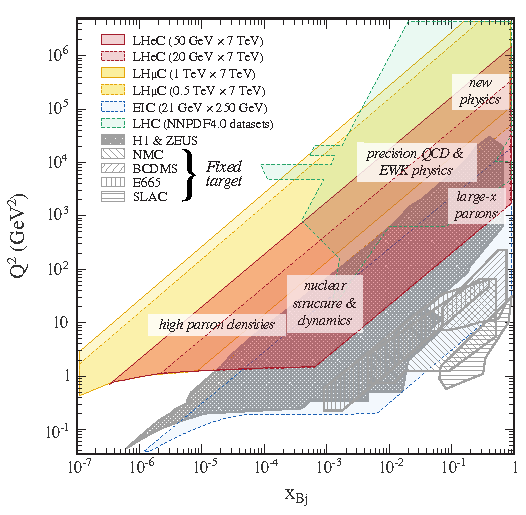
\includegraphics[width=.85\textwidth]{xbjq2_diagram.pdf}
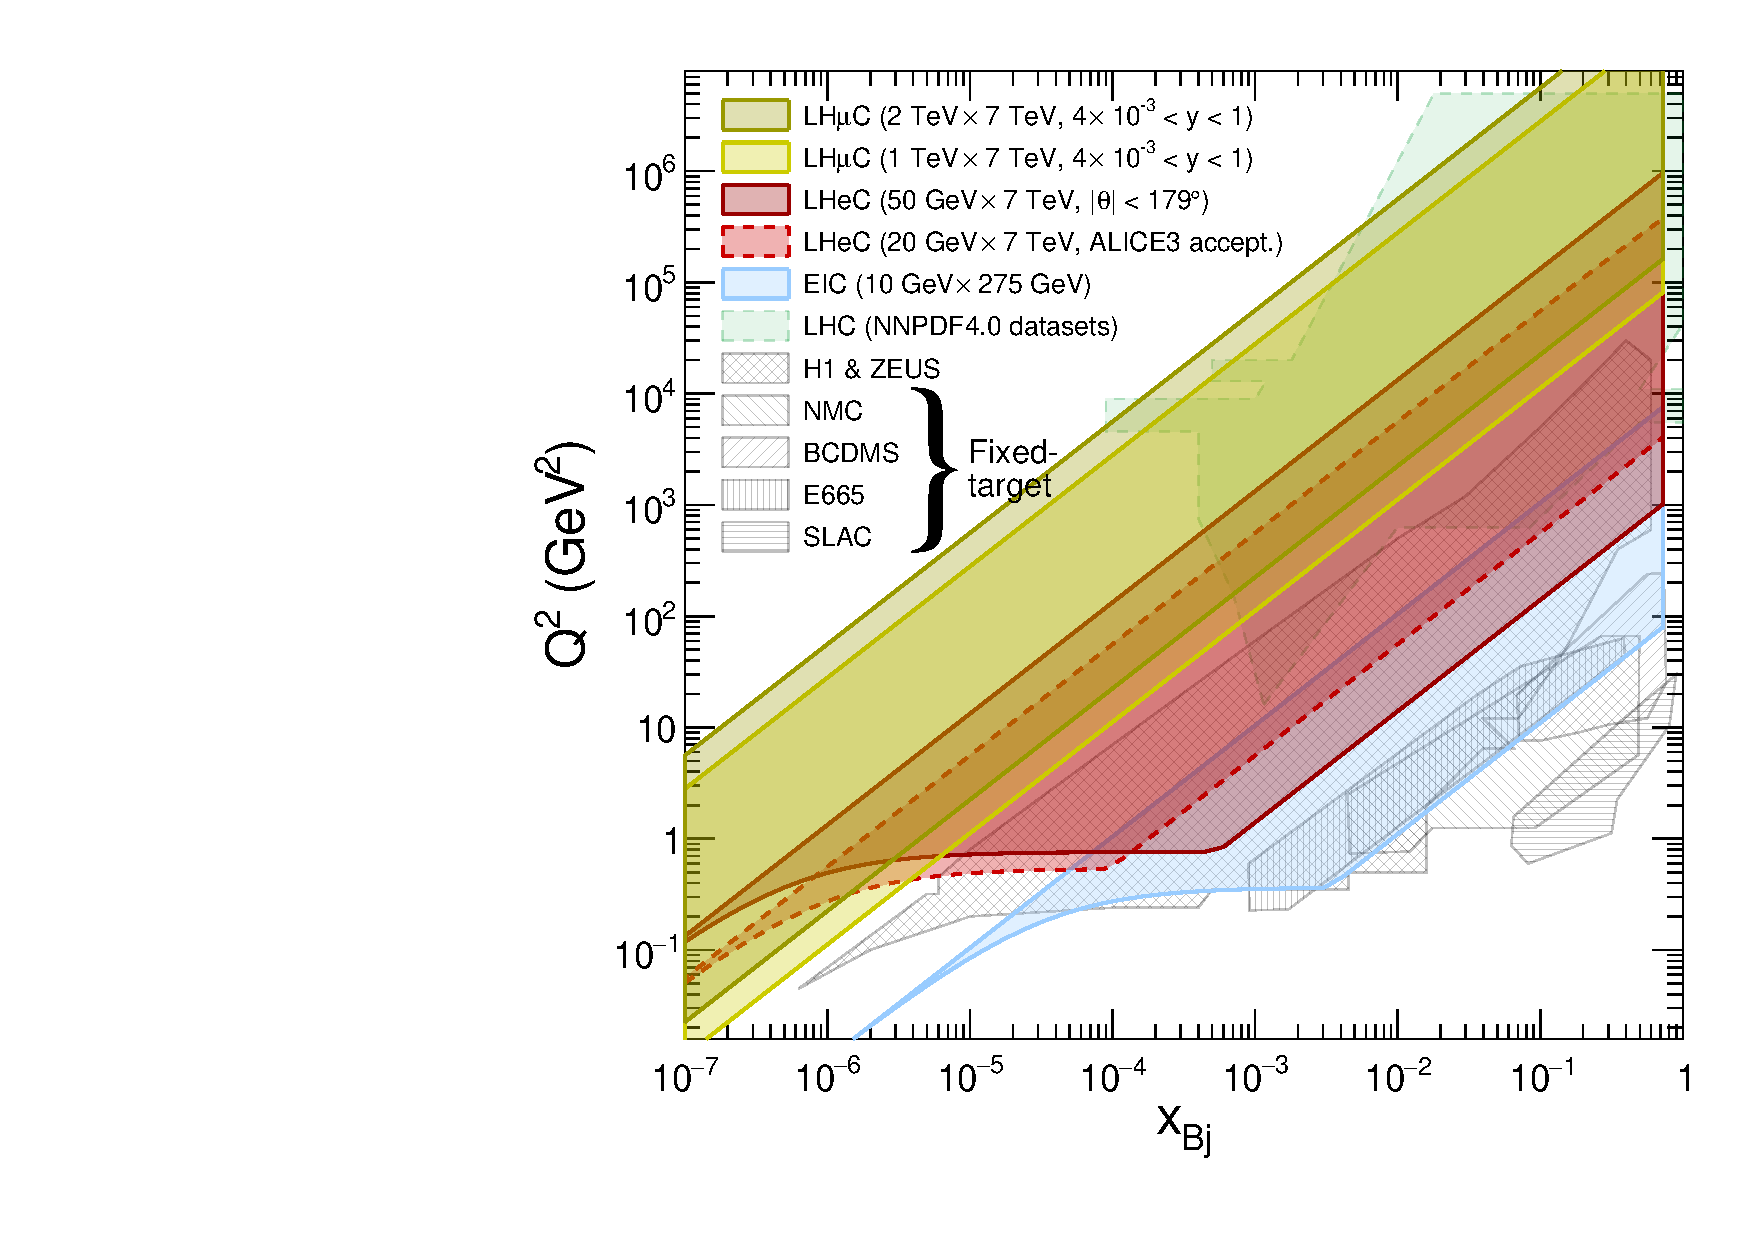
\includegraphics[width=.85\textwidth]{dis_eta_acceptance.pdf}
\caption{Available $(x,Q^2)$ plane for the proposed LHeC and \lhuc, in comparison to existing fixed target and collider datasets, and planned EIC kinematics reach. An inelasticity range of $4\cdot 10^{-3}<y<1$ is assumed to evaluate the lower and upper bounds.}
\label{fig:xbj_vs_q2_phase_space}
\end{figure}

\subsubsection{Non-linear QCD}

The QCD theory predicts that at fixed transverse resolution scale the gluon density in a hadron exhibits a fast power-like growth with decreasing $x_{\mathrm{Bj}}$, which eventually is tamed due to the nonlinear Yang-Mills field equations  \cite{Gribov:1984tu,Mueller:1985wy,McLerran:1993ni,Balitsky:1995ub,Kovchegov:1999yj}.
At sufficiently low $x_{\mathrm{Bj}}$ most gluons in the target carry transverse momenta of the order of a new dynamically generated large scale, the so-called saturation scale $Q_s(x)$. The key features of this state are: (i) the growth of the gluon density is tamed, both as a function of of $1/x$ and transverse momenta $k_T$ ($\log{(Q_s^2/k_T^2)}$ instead of $1/k_T^2$ for $k_T\ll Q_s$), (ii) relatively large transverse momenta of gluons tend to decorrelate the final state hadrons, (iii) the saturation scale, and thus the gluon density is enhanced by the mass of the target, roughly $Q^2_s(x)\sim A^{1/3}$ for large nucleus~\cite{Jalilian-Marian:2005ccm,Gelis:2010nm,Albacete:2014fwa,Blaizot:2016qgz}, therefore the cross section for nuclear targets are expected to be suppressed (per nucleon) compared to proton target.

Despite some aspects of the low-$x$ data of HERA, RHIC and LHC may indeed be described using the saturation models, the common belief is that the true gluon saturation effects still await a true discovery. The main reasons being: (i) the data does not explore the $x$ regime small enough, so that other nuclear effects contribute, (ii) the observable is too inclusive to discriminate saturation and non-saturation models. 

In what follows we briefly summarize the current status. The first hints for gluon saturation were observed at HERA, with a success of the Golec-Biernat-W\"usthof (GBW) saturation model model to describe the inclusive DIS data \cite{Golec-Biernat:1998zce} and realization that the data exhibits a geometric scaling predicted by the saturation model \cite{Stasto:2000er}. 
Another hints come from early RHIC data, notably the suppression of the forward inclusive production of hadrons and two-particle correlations in $\mathrm{dAu}$ (per nucleon) vs $\mathrm{pp}$~\cite{BRAHMS:2004xry,STAR:2006dgg,PHENIX:2011puq} as a result of the gluon saturation, see eg. \cite{Kharzeev:2002ei,Jalilian-Marian:2005ccm,Dumitru:2005gt,Albacete:2010pg}. Such suppression was also observed in the more recent RHIC data on $\mathrm{pAl}$ and $\mathrm{pAu}$ \cite{STAR:2021fgw,Chu:2021hda}. At the LHC, the suppression in $\mathrm{pPb}$ data was observed in the inclusive hadron $p_T$ specta~\cite{LHCb:2022tjh,LHCb:2023kqs}, but although it is consistent with the LO Color Glass Condensate computation \cite{Lappi:2013zma} it has tensions with the full NLO result \cite{Mantysaari:2023vfh}. The saturation also seems to be indirectly visible \cite{Penttala:2024hvp} in $J/\psi$ photoproduction in ultra-peripheral $\mathrm{PbPb}$ collisions \cite{ALICE:2021gpt,ALICE:2023jgu,CMS:2023snh,ALICE:2014eof,LHCb:2014acg,ALICE:2018oyo,LHCb:2018rcm}. 
There are also some hints from the LHC jet production data. The forward inclusive jet energy deposit in$\mathrm{pPb}$ collisions measured by the CASTOR detector~\cite{CMS:2018yhi} seems to indicate large nuclear effects, but not really consistent with saturation models or Monte Carlos \cite{Bury:2017xwd,Mantysaari:2019nnt,Liu:2022ijp}. Finally, the dijet correlations in $\mathrm{pPb}$ and $\mathrm{pp}$ at forward rapidity bins measured by ATLAS~\cite{ATLAS:2019jgo} seems  consistent with the saturation model, provided the suitable resummation is included~\cite{vanHameren:2019ysa}.

In order to better understand the potential of the new high energy muon-hadron collider for saturation physics, let us briefly summarize the theoretical description of the scattering process.

Within the QCD theory, or more concretely its high energy effective approximation -- the Color Glass Condensate (CGC), a scattering of a lepton off a dense target is usually described in terms of two components: (i) a projectile light cone wave function that describes an amplitude of a photon fluctuating into the quark-antiquark dipole; (ii) the color field of the target, whose valence components (highly localized in the longitudinal direction and randomly distributed in the transverse plane) act as classical sources for the delocalized color field. The color $q-\bar{q}$ dipole scatters off that small "wee" partons carrying small longitudinal fractions of the hadron momentum. 
The interaction of the high energy quark (or other parton emitted by the dipole) with the color field is -- in the eikonal approximation -- described by the straight infinite Wilson line along the light cone, at fixed transverse position. Eventually the product of the Wilson lines corresponding to the particular process has to be averaged with the distribution of the color sources. These \emph{Wilson line correlators} encode both the non-perturbative aspects of the color field distribution in the target, as well as the saturation phenomenon. 

The most basic correlator, relevant for inclusive DIS process, contains two Wilson lines and describes inclusive scattering amplitude for a color dipole. It can be related to the leading twist TMD gluon distribution, which is consequently called the \emph{dipole gluon distribution}. Interestingly, this distribution \emph{is not} the one appearing in the description of $p_T$ spectra of the Drell-Yan process.

\subsubsection{PDFs at low $x$}
full flavor decomposition in PDFs etc.

\subsubsection{Hard QCD: from low to high scales}
A central objective of the \lhuc physics program is high-precision tests of quantum chromodynamics (QCD), in particular the determination of the strong coupling constant $\alpha_s$ over an large range of momentum scales. QCD is a non‑Abelian gauge theory whose interaction strength decreases at short distances and increases at long distances, leading to a pronounced scale dependence of the strong coupling. 
A precise and consistent determination of the strong coupling $\alpha_s$ from low to very high momentum scales is essential, both for validating the internal consistency of QCD and its perturbative description, and as a key input to precision phenomenology at hadron colliders.

The \lhuc provides an excellent environment for precision QCD studies based on various neutral-current DIS measurements. Inclusive DIS measurements allow the extraction of
$\alpha_s$ through scaling violations of structure functions and global PDF fits. Jet production in the Breit frame provides a complementary and more direct sensitivity to
$\alpha_s$, while event‑shape observables probe
$\alpha_s$ in the hard perturbative region and through resummation effects.

%Owing to the clean DIS final state and the reduced QED initial- and final-state radiation associated with muon beams, systematic uncertainties are expected to be smaller than in electron–proton collisions. 
%Precise measurements can be performed at low scales, $Q \sim 3–5\,\text{GeV}$, ...

At higher momentum transfers, jet production in DIS provides a complementary and direct sensitivity to $\alpha_s$. 
Jet cross sections receive leading-order contributions from boson–gluon fusion and QCD Compton scattering diagrams, which are directly proportional to $\alpha_s$. 
Measurements of inclusive jet, dijet, and multijet cross sections over a wide kinematic range allow therefore for a direct determinations of $\alpha_s$. 
Dedicated measurements of three‑ and four‑jet cross sections exhibit an even stronger sensitivity to
$\alpha_s$, scaling already at leading order as $\alpha_s^2$ and $\alpha_s^3$, respectively.

TODO...

%at scales extending to the TeV range, with reduced dependence on non-perturbative effects.
%Studies for the LHeC indicate that uncertainties at the level of 0.2\% on αₛ are achievable from jet observables or inclusive DIS; the higher center-of-mass energy and luminosity of the LHµC are expected to further extend the accessible scale range.
%Additional constraints on αₛ can be obtained from event-shape observables in DIS, such as 1-jettiness. In particular, the region of small event-shape values is sensitive to logarithmically enhanced contributions that can be resummed to high perturbative accuracy. These measurements probe αₛ in a theoretically well-controlled resummation regime and provide an important cross-check of extractions based on inclusive and jet observables. Taken together, inclusive DIS, jet production, and event-shape measurements enable a determination of the strong coupling over scales ranging from a few GeV up to O(1–3 TeV), corresponding to roughly half the available center-of-mass energy. This broad coverage allows a coherent test of QCD and its running coupling across nearly six orders of magnitude in scale within a single experimental framework.

\subsubsection{...}
\subsubsection{Nuclear effects and nPDFs}


\subsection{HET Factory}
\subsubsection{Higgs case}

[Simone, Simon, Kingman, Mukesh]\\

After the discovery of an SM-like Higgs boson at the LHC in 2012~\cite{ATLAS:2012yve,CMS:2012qbp}, one of the central topics in high-energy physics has been to test the properties of the Higgs boson, including its couplings to other SM particles.
Given the large production rates of the SM Higgs bosons at the proposed $\mu^+$-proton collider facilities, it is possible to measure the Higgs-boson couplings to other SM particles with relatively small uncertainties.

Here, following Ref.~\cite{Cheung:2021iev}, we estimate the measurement uncertainty of the Higgs-boson coupling to the $b$-quarks.
We generate the charged-current VBF process $p \mu^+\to j \, \bar{\nu}_\mu \, h$, with the SM Higgs boson $h$ subsequently decaying into a pair of $b$-quarks.
The dominant background processes are the multijet charged-current one $p\mu^+ \to \bar{\nu}_\mu j j j$ and the VBF $Z$-boson production followed by $Z\to b\bar{b}$.
The measurement uncertainty of the cross section of $p \, \mu^+\to j \, \bar{\nu}_\mu \, b\,\bar{b}$ reads as,
\begin{eqnarray}
    \Delta\sigma/\sigma=\sqrt{N_s+N_b}/N_s,
\end{eqnarray}
where $N_{s/b}$ denotes the signal/background event numbers and only the statistical error is included.
We generate the parton-level events with \mgamcnlo, requiring $p_T^{j/b}>5$~GeV and $|\eta^{j/b}|<5.5$; the two parton-level cuts avoid the collinear limit and correspond to the geometry of the LHeC detector (which we assume as employing the same design as the $\mu^+$-proton collider detectors).
We use Pythia~6.428~\cite{Sjostrand:2006za} to properly process the parton showering and hadronization for such proton-lepton asymmetric collisions.
Finally, we use FastJet~3.3.2~\cite{Cacciari:2011ma,Cacciari:2005hq} to perform jet clustering with the anti-$k_t$ algorithm~\cite{Cacciari:2008gp} and then Delphes~3.4.2~\cite{deFavereau:2013fsa} for fast detector simulation where we apply an LHeC Delphes card that has included the beam asymmetry.
We take a universal factor of $75\%$ for $b$-tagging efficiency.

We select events with exactly two $b$-jets and require that the invariant mass of the $b$-quark pair should be close to the Higgs-boson mass: $|m_{bb}-m_h|<25$~GeV.
The latter cut facilitates separation between the signal ($h$) and background ($Z$) events.
We then calculate the signal-event and background-event numbers with $N_s=\mathcal{L}_{\text{int}}\cdot\sigma(p\,\mu^+\to j \,\bar{\nu}_\mu\,h)\cdot \text{BR}(h\to b\bar{b})\cdot \epsilon^{\text{sig}}_{\text{cut}}$ and $N_b=\mathcal{L}_{\text{int}}\cdot\Big(\sigma(p\,\mu^+\to j \,\bar{\nu}_\mu\,Z)\cdot \text{BR}(Z\to b\bar{b})\cdot \epsilon^{\text{bgd}-Z}_{\text{cut}}+ \sigma(\mu^+\to \bar{\nu}_\mu j j j )\cdot \epsilon_{\text{cut}}^{\text{bgd}-\text{m}j}\Big)$, where $\epsilon^{\text{sig}}_{\text{cut}}$ is the cut efficiency on the signal events and $\epsilon^{\text{bgd}-Z}_{\text{cut}}$ and $ \epsilon_{\text{cutn}}^{\text{bgd}-\text{m}j}$ are the cut efficiencies on the VBF-$Z$ and the multijet background events, respectively.
We find that for both proposed $\mu^+$-proton collider setups, $\epsilon^{\text{sig}}_{\text{cut}}$ is about $20\%$, and $\epsilon^{\text{bgd}-Z}_{\text{cut}}$ and $\epsilon_{\text{cut}}^{\text{bgd}-\text{m}j}$ are respectively about $2.5\%$ and $0.01\%$, and we obtain the sensitivity reach to $\Delta\sigma/\sigma$ to be $1.19\%$ and $0.69\%$ for the two collider setups, respectively.
In Table~\ref{tab:hbb} we list the signal and background event cross sections (with the parton-level cuts imposed) and cut efficiencies.
Note that here $\sigma_{\text{bgd}-Z}=\sigma(p\mu^+\to j \bar{\nu}_\mu Z)\cdot \text{BR}(Z\to b\bar{b})$. 

\begin{table}[htbp]
\centering
\begin{tabular}{lcccccc}
\hline
collider &  $\sigma_\text{sig}$ [pb] & $\sigma_{\text{bgd}-Z}$ [pb]  & $\sigma_{\text{bgd}-\text{m}j}$ [pb]  &  $\epsilon^{\text{sig}}_{\text{cut}}$    &  $\epsilon^{\text{bgd}-Z}_{\text{cut}}$  & $\epsilon^{\text{bgd}-\text{m}j}_{\text{cut}}$ \\
\hline 
$\mu p$-1 & 0.24 &  0.30 &  357.9 & 0.22  &0.025  & $9.7\times 10^{-5}$  \\
$\mu p$-2 & 0.39 & 0.50 &  563.8 & 0.21  & 0.025 &  $1.23\times 10^{-4}$ \\
\hline
\end{tabular}
\caption{Signal and background cross sections and cut efficiencies.}
\label{tab:hbb}
\end{table}


In order to proceed to compute the uncertainties on the measured Higgs coupling with the $b$-quarks, we should take into account the measurement uncertainties on $g_{hWW}^2/\Gamma_h$ where $g_{hWW}$ and $\Gamma_h$ are the Higgs coupling to the $W$-bosons and its total decay width, respectively.
$\Delta\left({g_{hWW}^2}/{\Gamma_h}\right)/\left({g^2_{hWW}}/{\Gamma_h}\right)$ is estimated in Ref.~\cite{Cheung:2021iev} to be $0.985\%$.
Now, since $\sigma(p\,\mu^+\to j \, \bar{\nu}_{\mu}\, b\, \bar{b})=\sigma(p\,\mu^+\to j \, \bar{\nu}_{\mu}\, h)\cdot \text{BR}(h\to b\bar{b})\sim{g^2_{hWW}\cdot g^2_{hbb}}/{\Gamma_h}$, we calculate the uncertainty on $g_{hbb}$ with 

\begin{eqnarray}
%\begin{displaymath}
\frac{\Delta g_{hbb}}{g_{hbb}}=\frac{1}{2}\sqrt{\left(\frac{\Delta\sigma}{\sigma}\right)^2+\left(  \frac{\Delta\left({g_{hWW}^2}/{\Gamma_h}\right)}{{g^2_{hWW}}/{\Gamma_h}}\right)^2}.
%\end{displaymath}
\end{eqnarray}

We find uncertainties of $0.77\%$ and $0.60\%$ can be achieved by the two proposed $\mu^+$-proton colliders, respectively.
These results surpass that expected at the LHeC ($0.97\%$)~\cite{lhecKappahbb} and the HL-LHC ($4\%$)~\cite{CMS:2013xfa,Cepeda:2019klc}.

It is worth noting that the $\mu p$-1 collider configuration is expected to test the Higgs-bottom-quark coupling with a precision better than the LHeC can, despite the smaller number of the Higgs-to-bottom-quarks decays at $\mu p$-1.
This is primarily due to the higher cutflow efficiencies on the signal events in this study than in Ref.~\cite{lhecKappahbb}.


\subsubsection{Higgs coupling global fit}

In order to asses the reach of LH$\mu$C in the Higgs sector we perform a simultaneous fit on the Higgs signal strength (SS) in the kappa-3 framework \cite{deBlas:2019rxi,deBlas:2022ofj}. The uncertainties on the Higgs SS in the LHeC white paper\cite{LHeC:2020van} are computed  from the statistical uncertainties multiplied by a systematical scale factor
\begin{equation}
   f_i = \sqrt{\frac{1+\frac{B}{S}}{A\cdot \epsilon} },
\end{equation}
depending on the background-signal ration, the acceptance and the efficiency rates.

In order to establish the LH$\mu$C reach in this first explorative study we assume the systematics factors to stay the same and rescale the statistical error using the cross-section compute in Tab. \ref{tab:i}.
The results of the kappa-3 fit expressed in terms of SM coupling modifiers, invisible and undetected branching ratios are shown in Fig. \ref{fig:kappafit} for different benchmark scenarios.
\begin{figure}[h]
\begin{center}
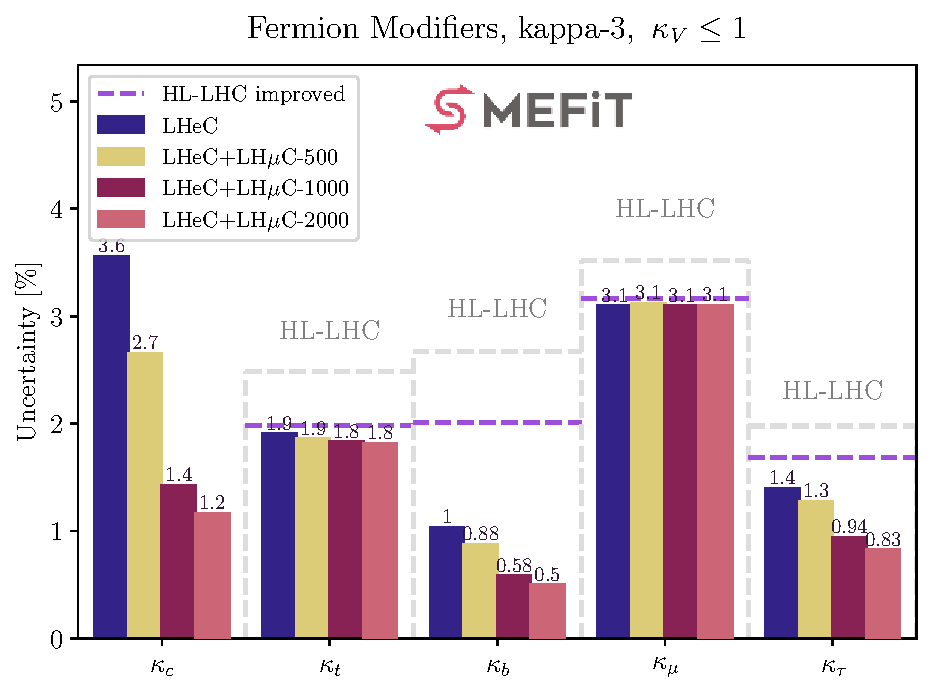
\includegraphics[width=0.49\textwidth]{LHmuC_fermion.pdf}
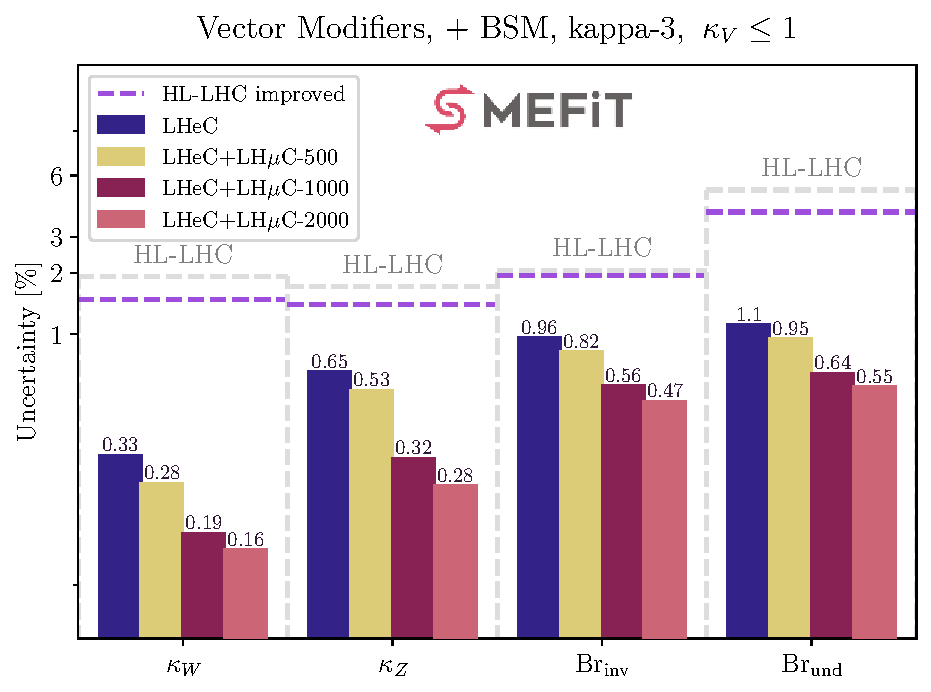
\includegraphics[width=0.49\textwidth]{LHmuC_vector.pdf}
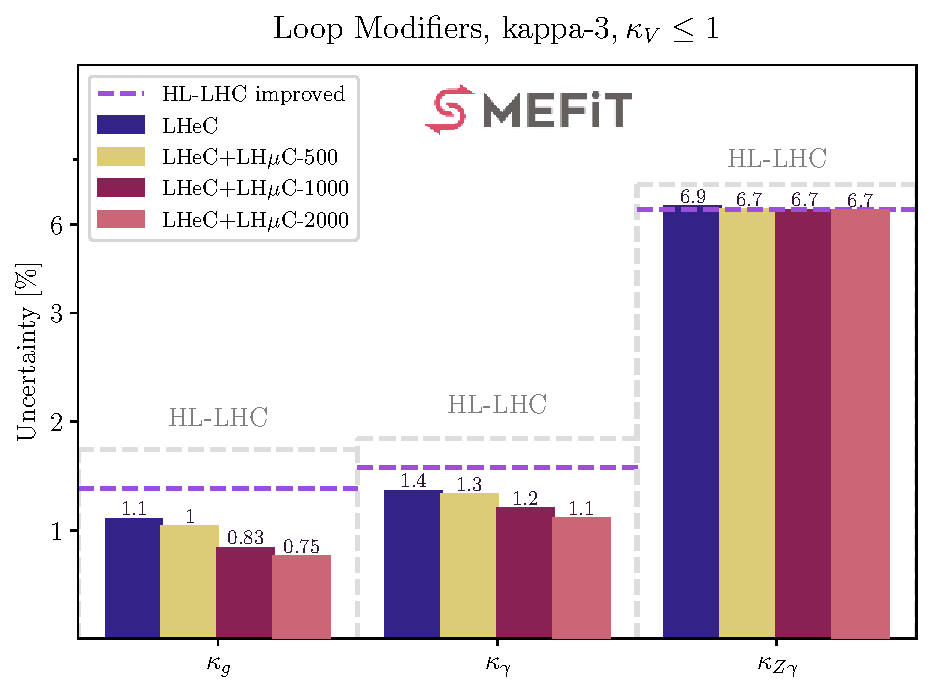
\includegraphics[width=0.49\textwidth]{LHmuC_loop.pdf}
\end{center}
\caption{Relative uncertainty in the coupling modifiers obtained in the kappa-3 framework~\cite{deBlas:2019rxi,deBlas:2022ofj}, for different combinations of the HL-LHC, LHeC, and LH$\mu$C stages. "HL-LHC improved" refers to the impact of reduced PDF+$\alpha_s$ uncertainties in the HL-LHC measurements as in \cite{Ahmadova:2025vzd}.  The fermion, vector, and loop modifiers are shown from top to bottom respectively. Since neither HL-LHC nor any $\ell p$ collider give direct access to the Higgs width, the condition $\kappa_V(\kappa_W, \kappa_Z)\le 1$ is imposed on the fit and the uncertainty on these modifiers is defined as $1-\kappa_V(68\%)$. Results have been obtained with the {\sc\small SMEFiT} framework~\cite{Armadillo:2026mvp}.
}
\label{fig:kappafit}
\end{figure}
For all \lhuc benchmarks, we take as baseline the HL-LHC projections \cite{atlas:2025eii} (gray dashed lines), as well as the same projections with $\alpha_s$ and PDF uncertainties reduced by the LHeC \cite{Ahmadova:2025vzd} (blue dashed lines), and the standalone LHeC performance. Although the Higgs production cross section increases when moving from LHeC to \lhmuc-500, the comparatively low luminosity of the latter significantly limits the achievable precision in Higgs coupling measurements.

In contrast, the \lhmuc-1000 and \lhmuc-2000 scenarios exhibit a substantial improvement in precision. In particular, $\kappa_W$ can be determined with a precision of $0.19\%$ and $0.16\%$, respectively, surpassing the reach of all other proposed future colliders, with the exception of a 10 TeV muon collider \cite{deBlas:2025gyz,Armadillo:2026mvp}.
No clear strategy have been ever proposed to measure independently the Higgs inclusive cross-section at $\ell p $ colliders, so in all the fits we assumed the additional condition $\kappa_V\le 1$ and define the uncertainty on these parameters as $1-\kappa_V(68\%)$, however we remind the reader that this condition can be explicitly broken by particular BSM scenarios \cite{Falkowski:2012vh}.


\subsubsection{Higgs self-interaction}

[Based of the contribution to the workshop]

%--------------------------------------------
\subsubsection{Precision electroweak physics}
%--------------------------------------------


highlights



\paragraph{$\sin^2{\theta_W}$:}
$\sin^2{\theta_\text{eff}}$ could become interesting with high integrated luminosity and high energy.








\paragraph{$m_W$:}

\paragraph{SMEFT parameters:}
Certain special SMEFT parameters could become interesting and are orthogonal to pp/ee.
Extrapolation of 2307.09459, like $C_{\phi W B}$ and $C^{(1)}_{\phi \ell}$ and $C_{\phi u}$


\paragraph{Tests of lepton universality?}



\paragraph{$\gamma\gamma$ physics at the LH$\mu$C:}\label{paragraph:twophoton}

The LH$\mu$C naturally operates as a high-energy photon-photon collider, where quasi-real photons radiated 
from the incoming muon and proton initiate exclusive $\gamma\gamma$ interactions. 
In the baseline configuration ($E_\mu=500~\mathrm{GeV}$, $\sqrt{s}\simeq 3.7~\mathrm{TeV}$), 
the effective $\gamma\gamma$ centre-of-mass energy could reach to the multi-TeV regime (up to $\sim 3~\mathrm{TeV}$), 
opening a broad programme of precision SM measurements and sensitive BSM searches 
in exceptionally clean final states.

A key feature is the very large rate of exclusive lepton-pair production, which provides both physics 
reach and powerful calibration handles. 
As a representative benchmark, the elastic $\gamma\gamma\to\tau^+\tau^-$ cross section is $\sigma_{\rm el}\simeq 58.56~\mathrm{pb}$ at the LH$\mu$C@3.7~TeV (to be compared with $\sim 50.37~\mathrm{pb}$ at the LHeC@1.2~TeV). 
For the 1~TeV muon upgrade ($\sqrt{s}\simeq 5.3~\mathrm{TeV}$), the corresponding elastic $\tau^+\tau^-$ rate 
increases further to $\sigma_{\rm el}\simeq 70.3~\mathrm{pb}$.
Hence, at the LH$\mu$C the corresponding rate is even larger 
yielding very high statistics within the central-detector acceptance.
This enables a competitive determination of the $\tau$ anomalous magnetic moment, $a_\tau$,
through precision measurements of the $\gamma\tau\tau$ vertex in $\gamma\gamma\to\tau^+\tau^-$ events,
including differential distributions and high-$m_{\tau\tau}$ tails where anomalous contributions are enhanced. 


Electroweak boson-pair production is another flagship channel. 
The elastic $\gamma\gamma\to W^+W^-$ rate rises from $\sigma_{\rm el}\simeq 0.037~\mathrm{pb}$ at the LHeC@1.2~TeV to $\sigma_{\rm el}\simeq 0.166~\mathrm{pb}$ at the LH$\mu$C@3.7~TeV, and to $\sigma_{\rm el}\simeq 0.258~\mathrm{pb}$ at $\sqrt{s}\simeq 5.3~\mathrm{TeV}$. 
The enhanced high-mass tail at higher $\sqrt{s}$ strengthens shape-based sensitivity to anomalous quartic gauge couplings (EFT dim-8 operators) in $\gamma\gamma W^+W^-$ process. 

The LH$\mu$C also offers unique access to loop-induced electroweak processes such as $\gamma\gamma\to ZZ$, 
which is absent at tree level in the SM. The elastic $ZZ$ cross section increases 
from $\sigma_{\rm el}\simeq 0.046~\mathrm{fb}$ at the LHeC@1.2~TeV to $\sigma_{\rm el}\simeq 0.284~\mathrm{fb}$ 
at the LH$\mu$C@3.7~TeV (and $\sigma_{\rm el}\simeq 0.463~\mathrm{fb}$ at $\sqrt{s}\simeq 5.3~\mathrm{TeV}$), 
enabling precision studies of the SM loop contribution and enhanced sensitivity to 
neutral quartic gauge couplings in the high-mass regime.

Finally, heavier exclusive final states become increasingly accessible. For instance, 
elastic $\gamma\gamma\to t\bar t$ rises to $\sigma_{\rm el}\simeq 0.486~\mathrm{fb}$ at the LH$\mu$C@3.7~TeV (vs.\ $\sim 0.046~\mathrm{fb}$ at the LHeC@1.2~TeV), and the same framework extends to the exclusive production of BSM 
charged-particle pairs, such as higgsinos and sleptons.
The combination of high energy, large $\gamma\gamma$ luminosity, and clean exclusive event topologies makes the 
LH$\mu$C a powerful laboratory for both SM precision and BSM discovery in photon-induced reactions.







%--------------------------------------------
\subsubsection{Top factory}\label{subsubsec:topfactory}
%--------------------------------------------

The LH$\mu$C provides a high-statistics and experimentally clean environment for top-quark studies.
At leading order, inclusive charged-current single-top production reaches
$\sigma(\ell p\to \nu_\ell t+X)=21.26~\mathrm{pb}$ (36.77~pb) for $E_\mu=500~\mathrm{GeV}$ (1~TeV),
while neutral-current top-pair production amounts to
$\sigma(\ell p\to \ell\,t\bar t+X)=1.03~\mathrm{pb}$ (2.23~pb), see Table~\ref{tab:i}.
Compared to the 50~GeV LHeC option, these rates correspond to an increase by factors of
$\sim 7$--$13$ for single top and $\sim 30$--$70$ for $t\bar t$.
With an integrated luminosity ${\cal L}_{\rm int}$ (?), the expected event yields scale as
$N \simeq ??$, implying multi-million single-top samples already for ${\cal O}(???)$.
The absence of significant pileup and the typically high acceptance expected at lepton--hadron machines
further enhance the precision reach in top-quark observables. 





\paragraph{toponium:}




\paragraph{single top:}




\paragraph{top charge:}





\paragraph{Rare decays and FCNC searches:}

With multi-million top samples, the LH$\mu$C offers an excellent opportunity to search for rare top-quark processes,
including flavour-changing neutral current  (FCNC) transitions mediated by $\gamma t q$ and $Z t q$ couplings ($q=u,c$),
as well as rare decays such as $t\to q\gamma$, $t\to qZ$ and $t\to qH$ in a clean experimental setting.
Both production and decay channels can be exploited, using the characteristic lepton--hadron event topology
to suppress backgrounds and define control regions. 
%{\color{blue} Hamzeh: A dedicated sensitivity study is ongoing to translate the large statistics into projected limits on FCNC branching ratios and EFT coefficients.}






%--------------------------------------------
\subsection{Unique BSM searches}
%--------------------------------------------

Several experimental tensions motivate searches for physics beyond the Standard Model at high-energy colliders, pointing to the possible existence of new particles and interactions. Anomalies observed in precision measurements and in heavy hadron decays suggest that new dynamics may be present in the flavor sector and in interactions involving leptons and quarks or gluons. While such interactions can
also be probed at hadron colliders, lepton--hadron colliders offer a qualitatively distinct advantage by enabling the resonant (single) production of new states, thereby providing enhanced sensitivity to their couplings and quantum numbers.

The LH$\mu$C offers unique sensitivity to new physics scenarios that couple preferentially to second-generation leptons. In particular, it enables direct searches for a broad class of Beyond the Standard Model signatures, including

\begin{description}
\item[Leptoquarks.] Hypothetical bosonic states carrying both lepton and baryon quantum numbers, predicted in various extensions of the Standard Model such as grand unified and composite models, and capable of mediating lepton--quark transitions~\cite{Pati:1974yy, Buchmuller:1986zs}.

\item[Color-octet leptons.] Strongly interacting partners of the leptons arising in scenarios with fermion compositeness, commonly referred to as leptogluons~\cite{Sahin:2010dd, Acar:2016rsw}.

\item[Excited leptons.] Higher-mass replicas of
Standard Model leptons predicted in composite frameworks, whose interactions can be described by effective operators coupling excited and ordinary leptons to gauge bosons~\cite{Terazawa:1981eg, Hagiwara:1985wt, Caliskan:2017meb}.

\item[Squarks.] Scalar partners of quarks appearing in supersymmetric extensions of the Standard Model, particularly in scenarios with R-parity violation where squarks can be produced singly and decay into lepton--quark final states~\cite{Beenakker:1996ch}.

\item[Contact interactions.] effective four-fermion operators encoding the low-energy effects of heavy new states beyond the direct kinematic reach, leading to observable deviations in cross sections and angular distributions~\cite{Eichten:1983hw, H1:2011ije}.
\end{description}
In addition to direct searches, precise measurements of production cross sections and angular distributions provide complementary indirect sensitivity to heavy new physics scales.



\subsubsection{R-parity-violating supersymmetry}

Lepton-proton colliders may produce squarks on resonance, if $LQ\bar{D}$-type operators in R-parity-violating (RPV) supersymmetry (SUSY) are present.\footnote{See Refs.~\cite{Dreiner:1998mxa,Barbier:2004ez,Mohapatra:2015fua} for reviews on the RPV SUSY.}
Here, following Ref.~\cite{Cheung:2021iev}, we study the sensitivity reach of the proposed $\mu^+$-proton collider setups to the RPV couplings as functions of squark masses.


The superpotential of the minimal supersymmetric standard model (MSSM) can be extended with the following terms if RPV is assumed:
\begin{eqnarray}
    W_{\text{RPV}} =\epsilon_i L_i\cdot H_u + \frac{1}{2}\lambda_{ijk}L_i\cdot L_j \bar{E}_k + \lambda'_{ijk} L_i\cdot Q_j \bar{D}_k + \frac{1}{2}\lambda''_{ijk} \bar{U}_i \bar{D}_j \bar{D}_k,
\end{eqnarray}
where the first three sets of operators violate lepton number and the last set violates baryon number.
As mentioned in the previous paragraph, we focus on the $L_i\cdot Q_j \bar{D}_k$ operators and assume all the other operators are vanishing; this can be realized by, for instance, imposing a baryon triality $B_3$ symmetry~\cite{Ibanez:1991pr,Dreiner:2012ae}.


We consider both charged-current (CC) and neutral-current (NC) signal processes, $p\, \mu^+\to \bar{d} \, \bar{\nu}_\mu$ and $p\, \mu^+\to d\, \mu^+$, via couplings $\lambda'_{21k}$ and $\lambda'_{2j1}$ with an $s$-channel mediator $\tilde{d}_R^*$ and $\tilde{u}_L$, respectively.
For the mediator mass below (above) the considered center-of-mass energy of the collider setup, the mediator squarks are dominantly on-shell (off-shell), in the signal processes.
Further, the corresponding background processes are $p\, \mu^+ \to j\, \bar{\nu}_\mu(+j)$ and $p\,\mu^+\to j \, \mu^+(+j)$, for the CC and NC signal channels, respectively.


We simulate both signal and background events with \mgamcnlo, exploiting the RPV-MSSM UFO model file~\cite{Monteux:2016gag}, with the parton-level cuts $p_T^j>5$~GeV and $|\eta^j|<5.5$.
Then Pythia~6~\cite{Sjostrand:2006za} processes parton showering and hadronization, FastJet~3~\cite{Cacciari:2011ma,Cacciari:2005hq} performs jet clustering, and DELPHES~3~\cite{deFavereau:2013fsa} with the LHeC card simulates detector effects.


In the CC (NC) case, we turn on only one single RPV coupling $\lambda'_{21k}$ ($\lambda'_{2j1}$), and scan over both the squark mass and the corresponding RPV coupling.
The decay width of the $s$-channel squarks are automatically computed with \mgamcnlo.\footnote{For squark masses below the QCD scale, in principle R-hadronization effects should be taken into account; since this is not included in \mgamcnlo, the package sets the corresponding squark width to 0. We have revoked this setup in \mgamcnlo, enforcing it to compute the squark decay widths, keeping the R-hadronization unconsidered.}
We extract the present $(36~\text{fb}^{-1})$ and future $(3~\text{ab}^{-1})$ LHC bounds on these couplings from Ref.~\cite{Bansal:2018dge}.
For $\lambda'_{21k}$, we take the following present and projected bounds: $\lambda'_{21k}<0.090\frac{m_{\tilde{d}_{Rk}}}{1~\text{TeV}}+0.014$ and $\lambda'_{21k}<0.053\frac{m_{\tilde{d}_{Rk}}}{1~\text{TeV}}+0.029$.
The bounds on $\lambda'_{2j1}$ are either in the same order of magnitude, looser, or non-existent; so we conservatively choose to take the same bounds as those on $\lambda'_{21k}$ for the illustrative purpose of the present study.


For the background processes, we perform MLM jet merging~\cite{Mangano:2006rw}.
Note that in this approach we have ignored the subdominant interference effects between the signal and background processes.
Finally, for the reconstructed events, we require that the events should contain at least one jet and exactly one muon.
We then select only events with the $p_T$ sum of the two leading jets larger than certain thresholds (for events with only one jet we require that the $p_T$ of the single jet should be sufficiently large).

We compute the signal significance $S$ with $S=N_s/\sqrt{N_b}$ with $N_{s/b}$ denoting the signal/background-event numbers.
Parameter points predicting $S=2$ correspond to the exclusion limits at $95\%$ confidence level (C.L.).

\begin{figure}
\centering
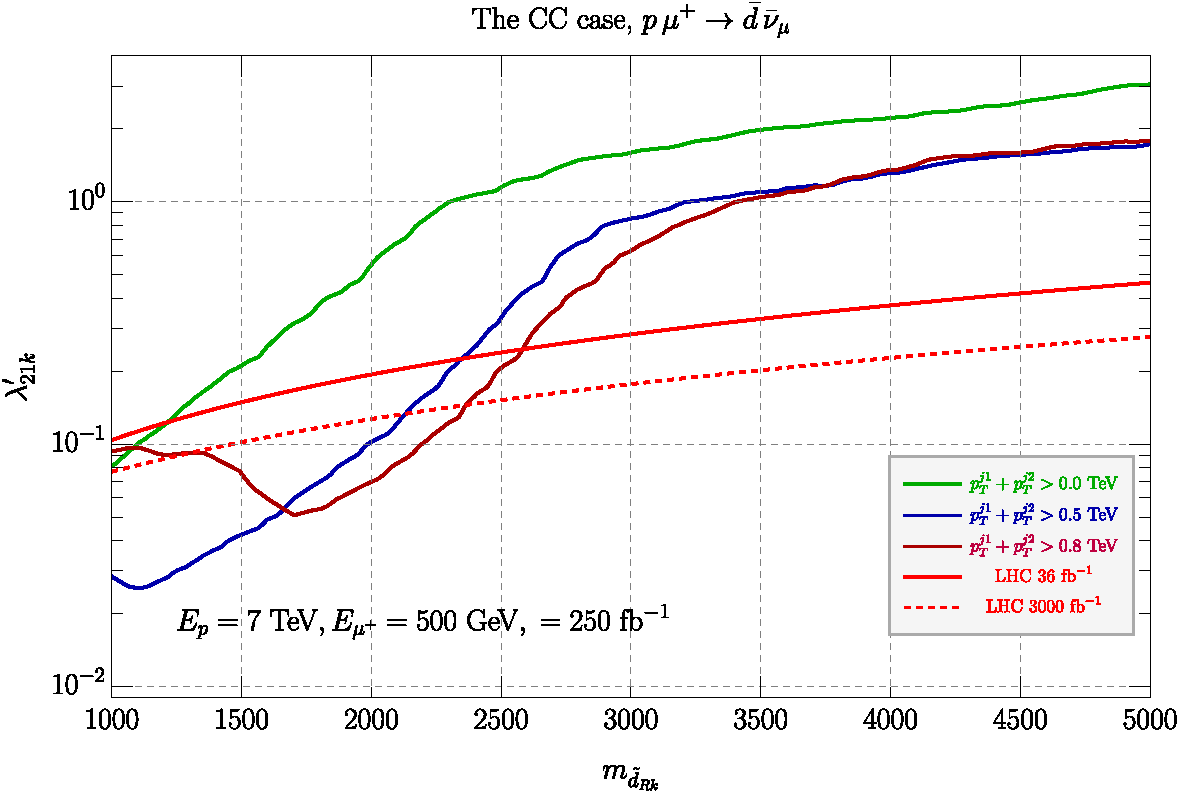
\includegraphics[width=.495\textwidth]{PlotSensitivity70p5_cc.pdf}
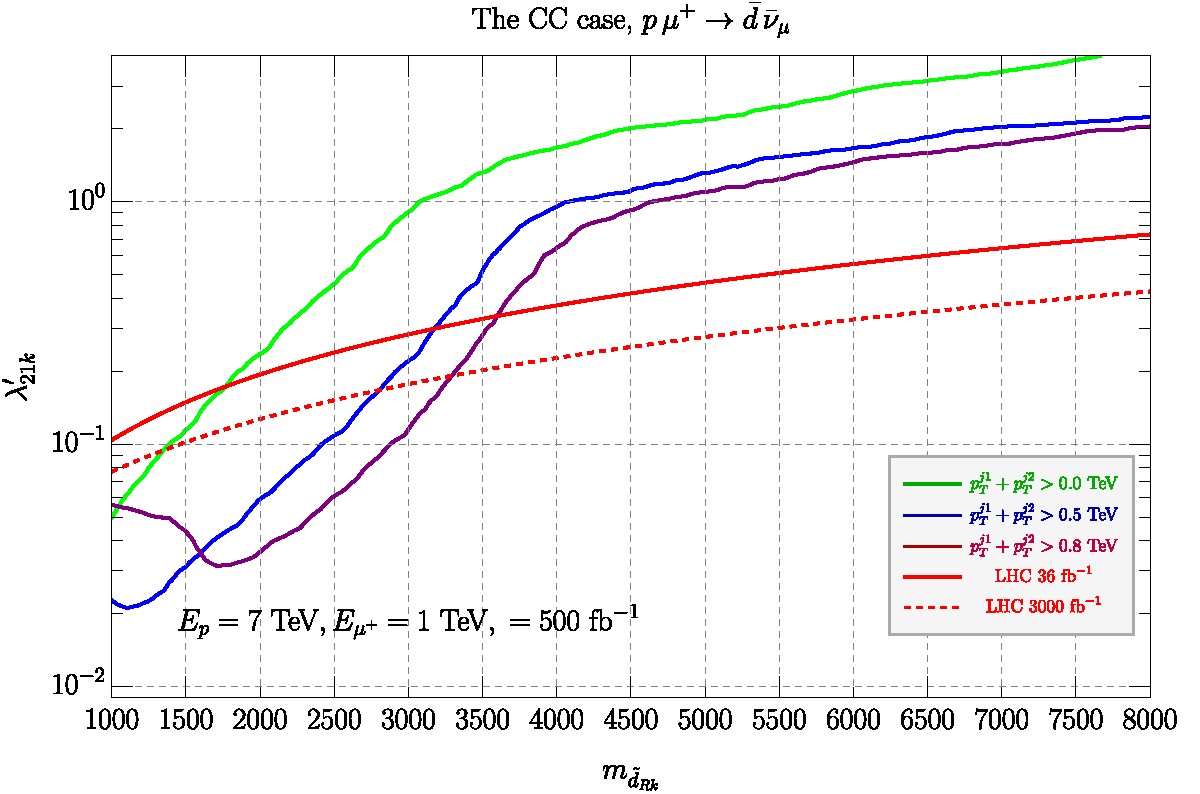
\includegraphics[width=.495\textwidth]{PlotSensitivity71_cc.pdf}
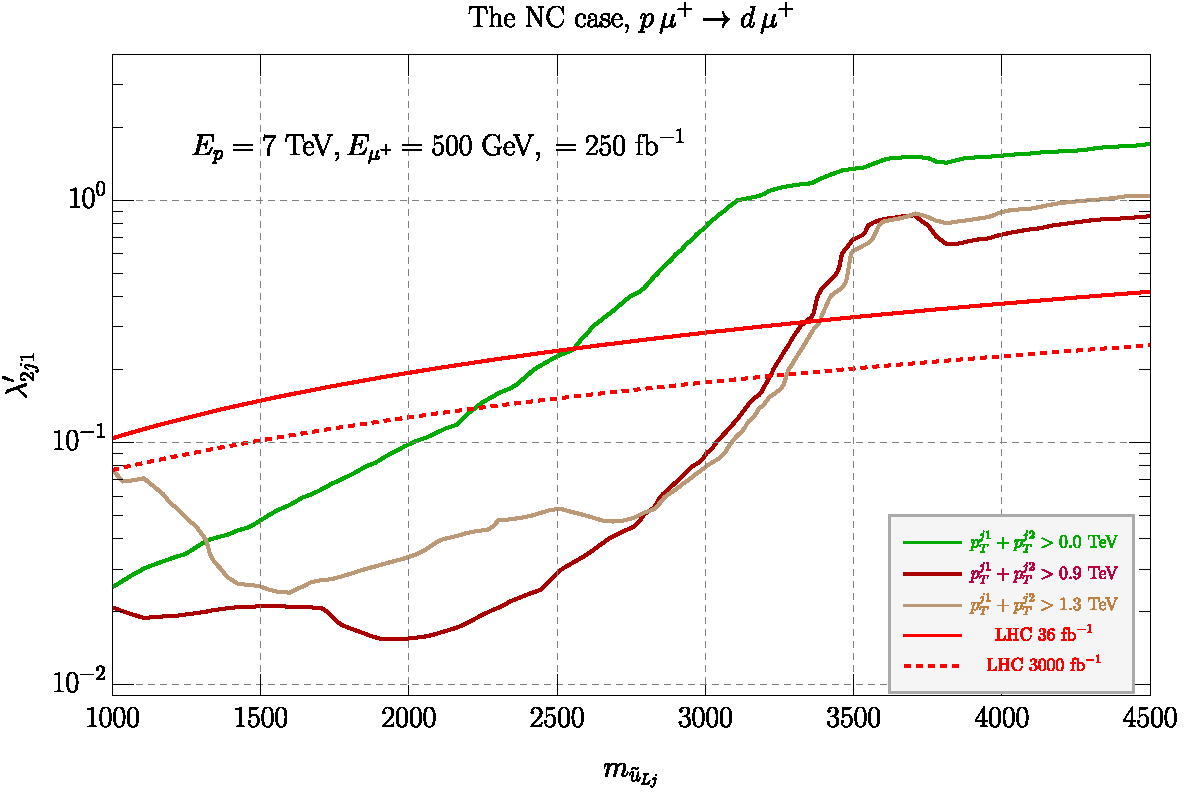
\includegraphics[width=.495\textwidth]{PlotSensitivity70p5_nc.pdf}
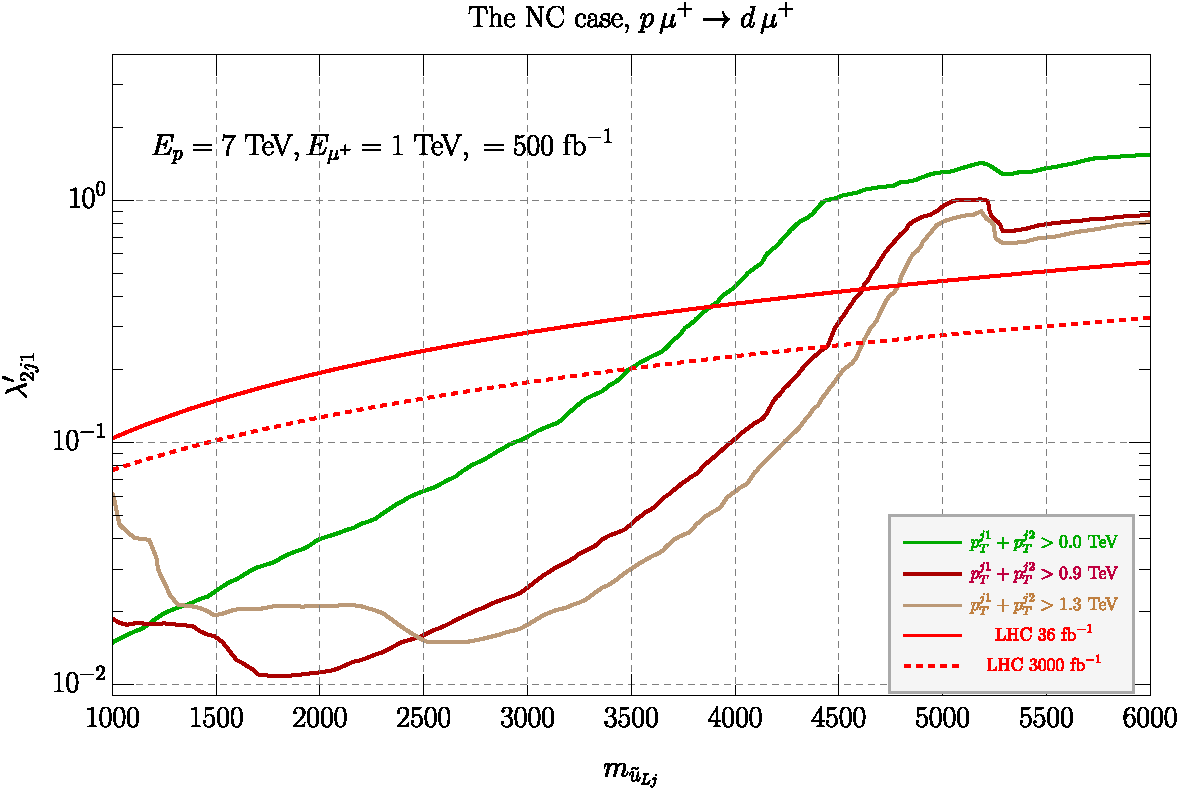
\includegraphics[width=.495\textwidth]{PlotSensitivity71_nc.pdf}
\caption{$95\%$ C.L.~exclusion limits on the considered RPV couplings as functions of the squark masses and the jet-$p_T$-sum thresholds we apply. The red curves are LHC bounds~\cite{Bansal:2018dge}.}
\label{fig:rpv_susy}
\end{figure}
We display the resulting sensitivity plots in Fig.~\ref{fig:rpv_susy}.
The upper and lower panels are for the CC and NC cases, respectively, and the left and right columns are for the two proposed $\mu^+$-proton collider setups, respectively.
Generally we observe that imposing a higher jet-$p_T$-sum threshold would render the search more sensitive to heavier squarks.
The two collider setups show similar sensitivities, and the sensitivities in the NC case are stronger than those in the CC case.
The latter is so because in the NC (CC) case a valence (sea) quark from the proton participates in the hard process.
In particular, we see that in the NC case the proposed $\mu^+$-proton colliders can test $\lambda'_{2j1}$ down to about 0.01--0.02 for squark masses 1--3~TeV, almost one order of magnitude stronger than the LHC bounds.


\subsubsection{Search for Color-Octet Muons}

Composite models of leptons and quarks provide an appealing extension of the Standard Model (SM) by suggesting that these particles may possess an underlying substructure composed of more fundamental constituents, commonly referred to as \textit{preons} \cite{DSouza:1992}. In several realizations of this paradigm, each SM lepton, which is a color singlet under SU(3)$_c$, is accompanied by a color-octet partner known as a leptogluon \cite{GoncalvesNetto:2013}. The color-octet muon, $\mu8$, carries a QCD color charge in the adjoint representation while sharing the same electroweak quantum numbers as the SM muon, making it a promising probe of lepton compositeness.

The effective interaction between leptogluons, Standard Model (SM) leptons, and gluons is described by a dimension-five operator suppressed by the compositeness scale $\Lambda$. The corresponding interaction Lagrangian is given by \cite{Acar:2018, Akturk:2025ubm}

\begin{eqnarray}
\mathcal{L} = \frac{1}{2\Lambda}
\left\{
\bar{l}_8^{\alpha} \, g_s \, G_{\mu\nu}^{\alpha} \,
\sigma^{\mu\nu}
\left( \eta_L \, l_L + \eta_R \, l_R \right)
+ \mathrm{h.c.}
\right\}.
\end{eqnarray}

Here, $g_s$ is the strong coupling constant, $G_{\mu\nu}^{\alpha}$ denotes the gluon field strength tensor with color index $\alpha$, and $l_8^{\alpha}$ represents the color-octet lepton field. The fields $l_L$ and $l_R$ correspond to the left- and right-handed components of the SM lepton field $l$, respectively. The tensor $\sigma^{\mu\nu} = \frac{i}{2}[\gamma^\mu,\gamma^\nu]$ is the antisymmetric Lorentz tensor, while $\eta_L$ and $\eta_R$ are dimensionless chirality factors governing the strength of the left- and right-handed couplings.

At proton--proton colliders, namely the LHC and its high-luminosity phase HL-LHC, the production of the color-octet muon, $\mu8$, proceeds predominantly through pair production mechanisms driven by strong interactions. In contrast, at muon--proton colliders, the direct $\mu g$ initial state allows for resonant single production of $\mu8$ via the process $\mu g \rightarrow \mu8$. Owing to the large gluon density inside the proton at high center-of-mass energies, this channel results in significantly enhanced production cross sections \cite{Akturk:2025ubm}. The representative production mechanisms for $\mu8$ at the HL-LHC and the LH$\mu$C are illustrated by the representative Feynman diagrams shown in Fig.~\ref{fig:mu8_feynman}.

\begin{figure}[htbp]
\centering
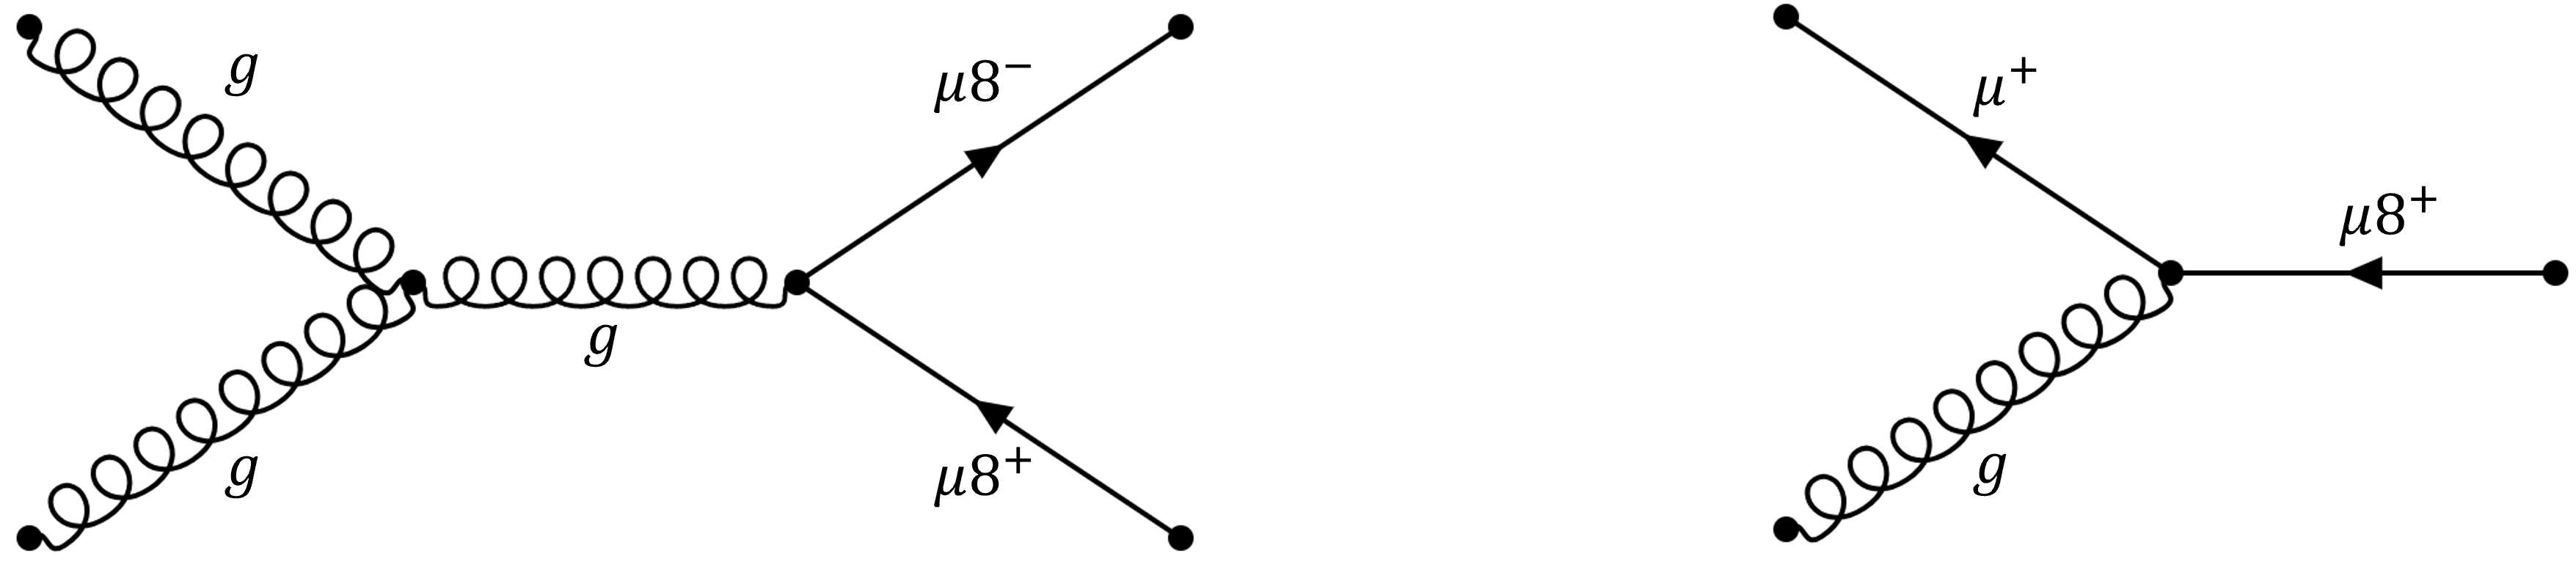
\includegraphics[width=.75\textwidth]{mu8_feynman.png}
\caption{Representative Feynman diagrams for $\mu8$ production: pair production at the HL-LHC (left) and single production at the LH$\mu$C (right).
\label{fig:mu8_feynman}}
\end{figure}

A hadron-level analysis is performed to evaluate the statistical significance of the $\mu8$ signal at the HL-LHC and the LH$\mu$C. In the signal samples, the produced $\mu8$'s are assumed to decay into a muon and a gluon. The dominant SM backgrounds are selected according to the final states of the corresponding signal channels: $\mu^+ p \rightarrow \mu^+ j$ for single production at the LH$\mu$C and $pp \rightarrow \mu^- \mu^+ jj$ for pair production at the HL-LHC. A total of 100k signal and background events are generated at parton level using \mgamcnlo~\cite{Alwall:2011}, employing the leptogluon model file named \textit{Leptogluon\_2ndgen\_UFO} \cite{Canbay:2025} prepared in \textsc{FeynRules} \cite{Christensen:2009}, followed by parton showering and hadronization with \textsc{Pythia8} \cite{Sjostrand2008}; jet clustering is performed using \textsc{FastJet} \cite{Cacciari:2011ma}, and the event analysis is carried out with \textsc{MadAnalysis5} \cite{Conte2013}.


The analysis is performed for $\mu8$ masses scanned over the range $m_{\mu8} = 1$--$6~\mathrm{TeV}$, while the compositeness scale is chosen as $\Lambda = m_{\mu8}$. For the LH$\mu$C single-production channel, events are required to contain exactly one muon and one jet in the final state. The transverse momentum distributions of the leading muon and jet peak around half of the $\mu8$ mass, reflecting the near-threshold production of the resonance. Motivated by this characteristic behavior, transverse momentum cuts of $p_T > 400~\mathrm{GeV}$ are applied to both the muon and the jet. In addition, pseudo-rapidity requirements of $|\eta_j| < 3.5$ for the jet and $|\eta_\mu| < 3$ for the muon are imposed to ensure central detector acceptance.

A parallel analysis is performed for pair production at the HL-LHC, where events with two muons and two jets are selected. The same pseudo-rapidity cuts are applied, while softer transverse momentum thresholds of $p_T > 300~\mathrm{GeV}$ for the leading muon and jet and $p_T > 250~\mathrm{GeV}$ for the subleading ones are used.

For the statistical analysis, the numbers of signal ($S$) and background ($B$) events are extracted from the invariant mass spectra after applying all selection cuts, assuming an integrated luminosity of $1~\mathrm{ab}^{-1}$ for the HL-LHC, while for the LH$\mu$C an integrated luminosity of $250~\mathrm{fb}^{-1}$ is used for the 500~GeV muon beam option and $500~\mathrm{fb}^{-1}$ for the 1000~GeV muon beam option. The statistical significance is evaluated as $\mathcal{S}=S/\sqrt{B}$, and the resulting significance values are shown in Fig.~\ref{fig:mu8_significance}.

\begin{figure}[htbp]
\centering
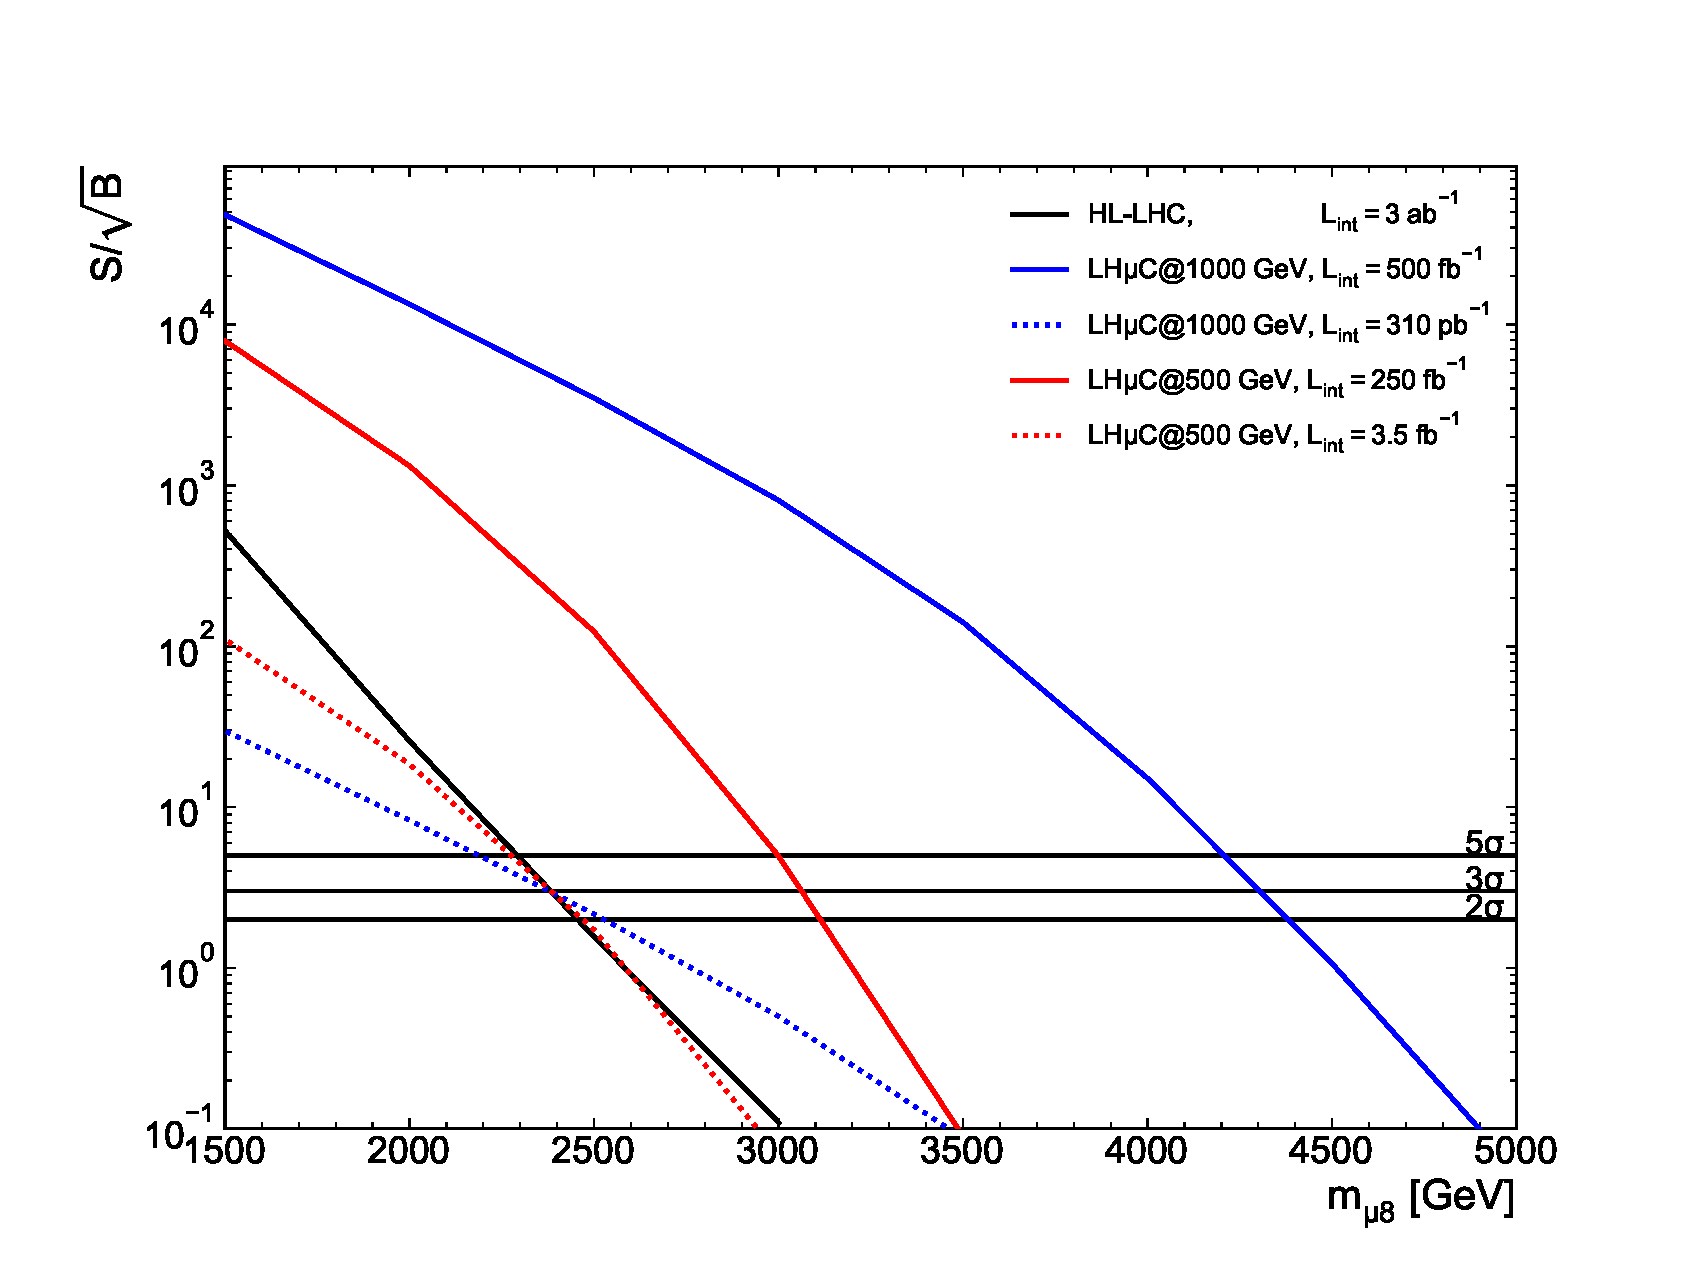
\includegraphics[width=.75\textwidth]{mu8_significance.eps}
\caption{Statistical significance of the $\mu8$ mass for the HL-LHC and the LH$\mu$C configurations.
\label{fig:mu8_significance}}
\end{figure}

As can be seen from Fig.~\ref{fig:mu8_significance}, the LH$\mu$C configurations provide a substantially higher sensitivity to $\mu8$ production compared to the HL-LHC. The $5\sigma$ discovery reach is found to be approximately $2.3~\mathrm{TeV}$ for the HL-LHC, while it extends up to about $4.2~\mathrm{TeV}$ for the LH$\mu$C with the 1000~GeV muon beam option and about $3.0~\mathrm{TeV}$ for the 500~GeV muon beam option. 

Moreover, when the $3\sigma$ significance criterion is considered, the LH$\mu$C is able to reach the HL-LHC discovery mass limit with considerably lower integrated luminosity. In particular, the same mass reach can be achieved with an integrated luminosity of approximately $3.5~\mathrm{fb}^{-1}$ for the 500~GeV option and about $310~\mathrm{pb}^{-1}$ for the 1000~GeV option, demonstrating the strong potential of the LH$\mu$C for probing higher $\mu8$ mass scales.


\subsubsection{Contact-interactions}


\subsection{Neutrino physics [Xianguo]}


\subsection{Outlook/next steps}


\newpage




\section{High energy, high luminosity lepton-hadron colliders}

[Burak, Frank, Krzysztof, Umit]\\

LHeC~\cite{LHeC:2020van}, Stage one~\cite{Andre:2025iar}, LHeC@IP2~\cite{Andre:2022xeh}, \lhuc~\cite{Akturk:2025ubm}, $\mu$TRISTAN~\cite{Hamada:2022mua}, ultra cold $\mu$~beam~\cite{Aritome:2024rlu}

\label{sec:LHcolliders}

\subsection{LHeC}
The Large Hadron electron Collider (LHeC)~\cite{LHeCStudyGroup:2012zhm,LHeC:2020van} was proposed as the ultimate upgrade of the High-Luminosity--Large Hadron Collider (HL-LHC) program. An Energy Recovery Linac (ERL) based accelerator delivers 50\,GeV high-intensity electron beams to collide with the HL-LHC proton or ion beams at centre-of-mass energies $1.2 (0.8)$\,TeV/nucleon, and luminosities around $10^{34(33)}$ cm$^{-2}$s$^{-1}$, for electron-proton ($ep$) and electron-nucleus ($eA$) collisions, respectively. The design presented in~\cite{LHeCStudyGroup:2012zhm,LHeC:2020van} focused on the concurrent operation of $ep/eA$ in one LHC interaction point and $pp/AA$ in the others (see also Ref.~\cite{Andre:2022xeh}). In view of the new LHC schedule, it was proposed that the project fits in the years between the end of the regular HL-LHC program (currently 2041) and the start of a new major collider at CERN~\cite{Ahmadova:2025vzd}. With 6 years of LHeC running stand-alone, a total integrated luminosity of 1\,ab$^{-1}$ could be collected in $ep$ collision mode, with $eA$ collisions integrated in the $ep$ runs. 

In that most recent proposal, the ERL with a circumference of a third of the LHC’s has been chosen as a baseline~\cite{Ahmadova:2025vzd}, allowing delivery of 60~GeV electron beams corresponding to the centre-of-mass energy of 1.3~TeV for electron-proton collisions.
\label{subsec:LHeC}

\begin{figure}[htbp]
\centering
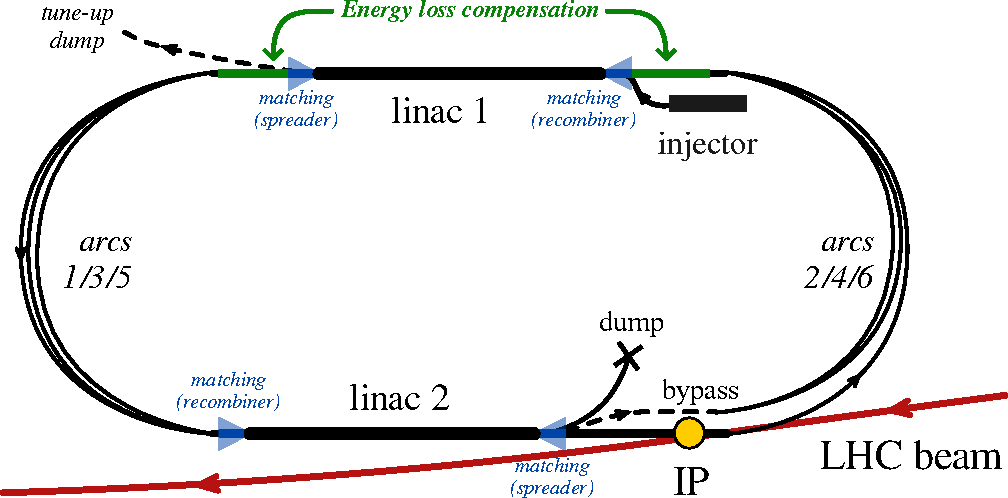
\includegraphics[width=.75\textwidth]{erl_schematics.pdf}
\caption{Layout of the proposed LHeC. The electron energy recovery linac (ERL) composed of two straight sections linacs interconnected by 2 triplets of return arcs are depicted in black, along with the electron injector, interaction region bypass, and beam dump. The proton storage ring hosting the LHC beam is depicted in red.\label{fig:lhec_schematics}}
\end{figure}

\subsubsection{Baseline LHeC}

In Fig.~\ref{fig:lhec_schematics} the layout of the baseline LHeC is presented -- an ERL of about 8.65~km circumference is composed of two linacs of 1.008~km length each, two sections of energy loss compensation having 230~m in total, six return arcs with a radius of 1~km and four matching sections of about 31~m each~\cite{LHeC:2020van}.

The nominal electron beam current is 50~mA and the lateral beam size at the IP is 4.8~$\mu$m, resulting in a nominal luminosity of $2.3\times10^{34}$ cm$^{-2}$s$^{-1}$ for electron-proton collisions~\cite{LHeC:2020van}.

\subsubsection{Stage-One LHeC}

To allow electron-hadron collisions during Run 5 of the HL-LHC program, Stage-One LHeC was proposed using a single-pass ERL to deliver 20~GeV electron beams, assuming its circumference of a third of the LHC’s, as above. For a nominal electron beam current of 60~mA and the lateral beam size at IP2 of 10.7~$\mu$m, one expects a nominal luminosity of $6\times10^{33}$~cm$^{-2}$s$^{-1}$ for electron-proton collisions at 0.75~TeV~\cite{Andre:2025iar}.

It is worth noting the possibility of running such a single-pass ERL in a standalone mode, i.e. without concurrent hadron-hadron collisions at the HL-LHC. In this case, the electron beam current of 150~mA and the lateral beam size at the IP of 4.8~$\mu$m can be considered, resulting in a very high luminosity in excess of $7\times10^{34}$~cm$^{-2}$s$^{-1}$. Moreover, using the space freed by unnecessary sections of energy loss compensation and by matching sections, additional RF cavities could be installed, allowing the electron beam energy to exceed 23~GeV. One can also consider a two-pass ERL delivering then a 46~GeV beam at the peak luminosity of about $4\times10^{34}$~cm$^{-2}$s$^{-1}$.

\subsection{\texorpdfstring{LH$\mu$C}{LHuC}}

The proposal for the LHµC arises as an evolution of the LHeC, designed to overcome the energy limitations imposed by synchrotron radiation in the electron sector. By transitioning to muons, it becomes possible to reach multi-TeV center-of-mass energies, which reinforces the argument for lepton-hadron colliders as a vital bridge project at CERN, maintaining its leadership at the energy frontier. However, the deployment of a high-energy muon beam introduces its own set of significant technical challenges. The International Muon Collider Collaboration (IMCC) has been dedicated to extensive R\&D about these challenges for a considerable period. 

The LH$\mu$C framework aims to leverage these global efforts while integrating the recently developed ultra-cold muon production method from J-PARC, instead of the conventional ionization cooling approach. By adopting this ultra-cold muon beam technology, we aim to integrate the subsequent acceleration system within the proposed LHeC layout at CERN. In the following subsections, we will first discuss the processes of high-intensity ultra-cold muon production and explore how the proposed LHeC infrastructure can be utilized for the rapid acceleration of muons. Subsequently, we will outline the design of an optimum main ring and interaction region, tailored to maximize the luminosity of muon-hadron collisions at the LH$\mu$C.

\label{subsec:LHuC}
\begin{figure}[h]
\centering
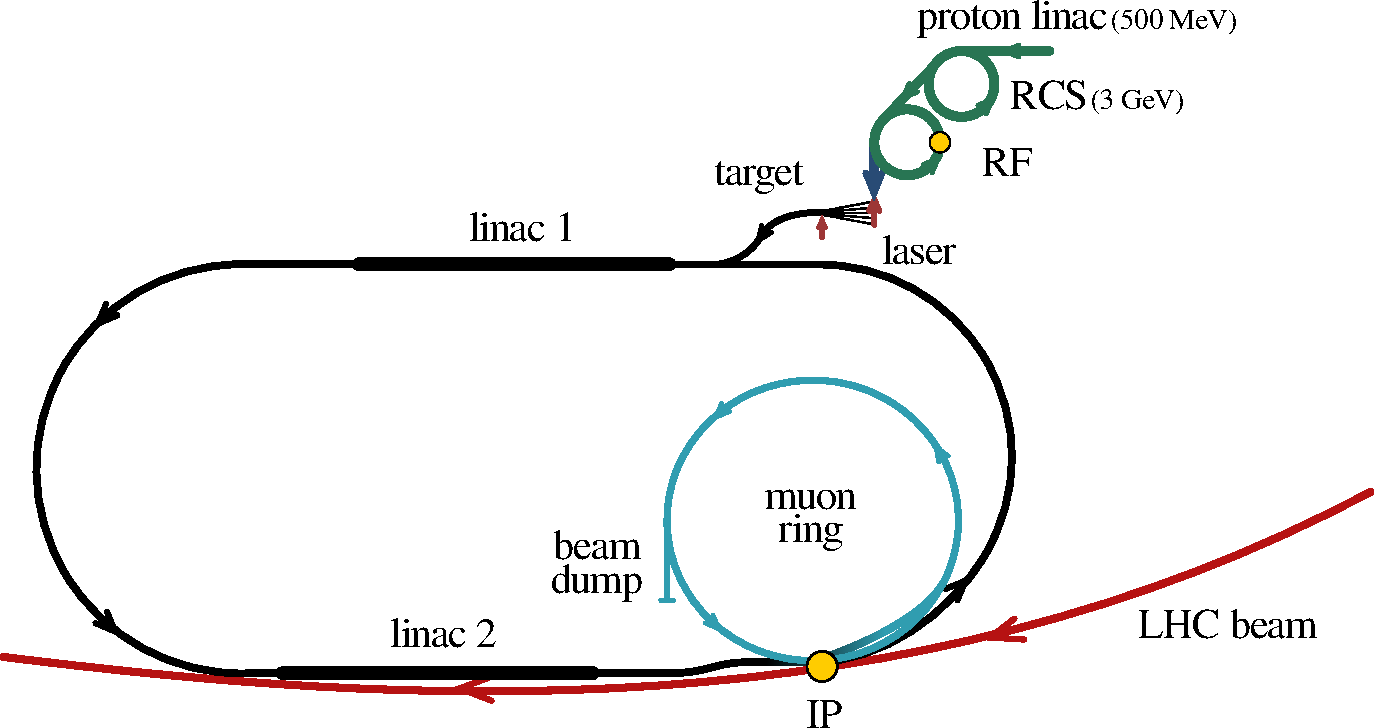
\includegraphics[width=.8\textwidth]{lhuc_schematics_v2.pdf}
%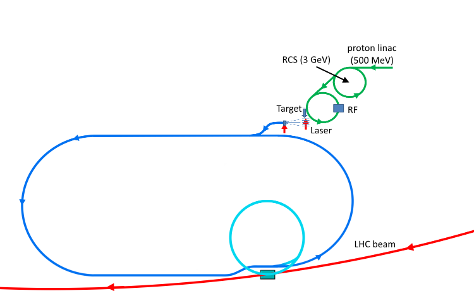
\includegraphics[width=.72\textwidth]{Picture 1.png}
\caption{Layout of the proposed \lhuc~\cite{Akturk:2025ubm}, based on the $\mu$TRISTAN proposal~\cite{Hamada:2022mua}. Following the same colour scheme as Fig.~\ref{fig:lhec_schematics}, the ERL components for the lepton beam circulation, and acceleration, are depicted in black, while the muon storage ring is shown in light blue along with its beam dump.\label{fig:i}}
\end{figure}

\subsubsection{Ultra cold \texorpdfstring{$\mu^+$}{muon}-source}


%Breakthrough at Muse/J-PARC~\cite{Aritome:2024rlu}


%%% some content - in preparation by Cedric

%Silica aerogel material for muonium emission was tested at TRIUMF~\cite{Bakule:2013poa} and laser-ablation on surface of aerogel was developed to increase the muonium emission by an order of magnitude~\cite{Beer:2014ooa}.

%Muon acceleration~\cite{Bae:2018atj,Aritome:2024rlu}

%Pulsed 122 nm laser for 1S-2P excitation.

%Breakdown of the efficiency of ultra-cold muon generation~\cite{Zhang:2021cba}. Novel multi-layer design~\cite{Zhang:2022ilj,Hamada:2022mua}

%%% references - in preparation by Cedric

%~\cite{Bakule:2013poa}
%~\cite{Beer:2014ooa}
%~\cite{Hamada:2022mua}
%~\cite{Bae:2018atj}
%~\cite{Aritome:2024rlu}
%~\cite{Zhang:2021cba}
%~\cite{Zhang:2022ilj}



The standard framework for muon production is based on the interaction of a high-power proton driver with a stationary target, typically graphite. This process generates pions that subsequently decay into muons. Since the resulting muon beam has a very large phase-space volume, the conventional approach relies heavily on ionization cooling to reduce the beam emittance. As outlined in current Muon Collider (MC) design studies~\cite{Delahaye:2019omf}, this involves a complex and resource-intensive "Front-End" system, including 6D rectilinear cooling and final cooling stages, to prepare the muon beam for acceleration.

However, the design of MC relies on ionization cooling, a complex process that imposes extreme technological demands. Cooling must occur extremely rapidly to counteract the muon’s short lifetime, requiring sophisticated wedge absorbers and high-gradient RF cavities operating within intense magnetic fields. Specifically, the final cooling stage requires solenoids capable of generating magnetic fields reaching up to 40 T. Consequently, the realization of this conventional scheme hinges on the successful development and widespread deployment of advanced High Temperature Superconductor (HTS) magnets. With the construction of a cooling demonstrator scheduled for 2035 at the earliest, these timeline and technological constraints motivate the search for alternatives.

To circumvent these complexities, the LHµC proposal adopts an alternative strategy based on the ultra-cold $\mu^+$ production technology recently advanced at J-PARC~\cite{Aritome:2024rlu}. While this method also begins with a proton driver and a primary production target, it diverges significantly by utilizing a laser-ionization process of thermal muonium atom-like structures. The conceptual layout of this muon source and the multi-step production chain of ultra-cold muon beam is illustrated in Figure~\ref{fig:mucooling}.

\begin{figure}[h]
\centering
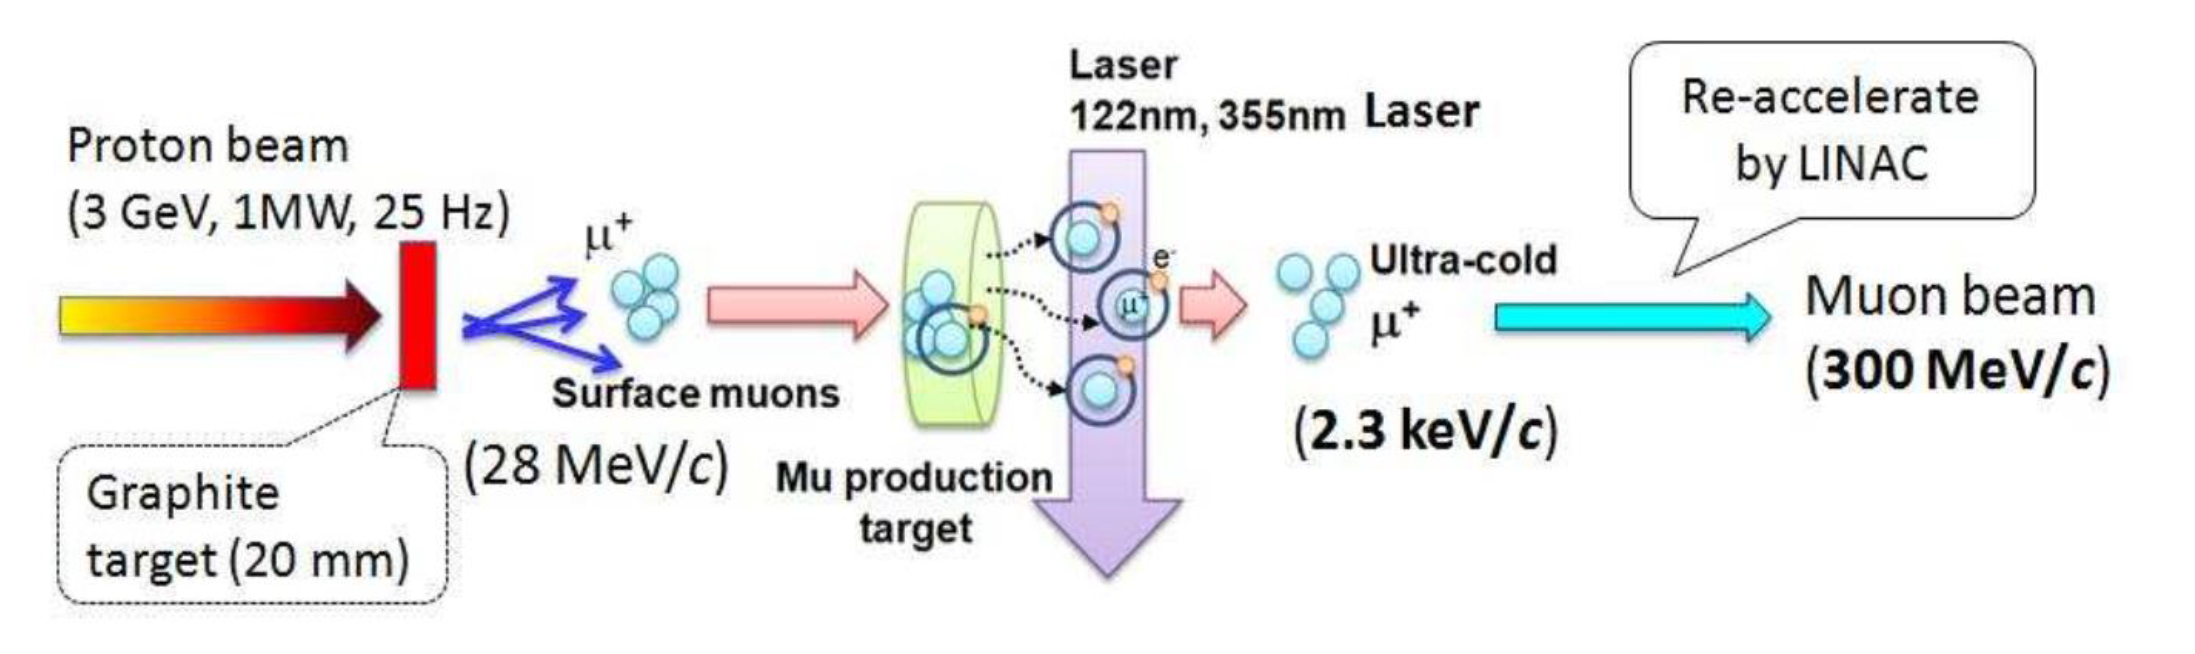
\includegraphics[width=1\textwidth]{J-PARC_cooling.png}
\caption{J-PARC ultra-cold muon beam production scheme.\label{fig:mucooling}}
\end{figure}

\textcolor{red}{The system utilizes a 3 GeV proton beam consisting of two bunches}, each carrying a charge of $6.6 \, \mu\text{C}$ (approximately $4.1 \times 10^{13}$ protons per bunch). Operating at a repetition rate of 25 Hz, this configuration delivers a total beam power of 1 MW ($3 \, \text{GeV} \times 6.6 \, \mu\text{C} \times 2 \, \text{bunches} \times 25 \, \text{Hz}$). This established high-power driver provides the necessary primary proton flux to initiate the high-yield muon production chain.

This approach generates an inherently ultra-cold positive muon beam with exceptionally low emittance. The process begins with the generation of surface muons ($28\,\mathrm{MeV}/c$) from the decay of pions stopped at the near surface of the graphite target. These positive muons are then directed onto a light target such as silica aerogel, where they slow down and capture electrons to form thermal muonium ($\mu^{+}e^{-}$) atoms. Laser-ablation has been implemented on the target surface to enhance the Muonium emission rate~\cite{Beer:2014ooa}. Muoniums diffuse into the vacuum region and are subsequently ionized via high-intensity Lyman-$\alpha$ lasers. The resulting "ultra-cold" muons possess extremely low transverse momentum, yielding a beam with normalized emittance at the level of a few mm·mrad. Finally, these ultra-cold muons are injected into a dedicated linac for initial re-acceleration, preserving their low emittance. 

\textcolor{blue}{In the J-PARC configuration, a single graphite target is used for pion production. The produced pions have a very broad momentum distribution, and only a limited momentum range can be efficiently captured by the extraction system. As a result, only a small fraction of the produced pions is utilized, for example for surface muons and decay muons originating from pions decaying in flight.} It is estimated that a muon rate increase of $10^5 - 10^6$ can be achieved at J-PARC through the implementation of a dedicated and optimized production chain~\cite{Zhang:2021cba}.

A prominent example of this development is the $\mu$TRISTAN proposal~\cite{Hamada:2022mua}, which aims to leverage a J-PARC proton accelerator–like facility together with the TRISTAN infrastructure to provide a roadmap for high-yield ultra-cold positive muon beams in $e^{-}\mu^{+}$ and $\mu^{+}\mu^{+}$ collider configurations. This enhancement is primarily achieved by implementing a separate pion production target followed by a multi-layered stopping target system, as illustrated in Figure~\ref{fig:multilayer}. Unlike the standard J-PARC setup, the majority of pions that bypass the initial graphite target are transported to a massive 10-meter-long system consisting of one thousand layers of 1 mm-thick tungsten foils. When accounting for the natural decay lifetime of the pions and the unavoidable losses due to scattering and material interactions during transport, the overall efficiency of successfully delivering and stopping the pions in the tungsten target is estimated to be $50\%$. 

\begin{figure}[h]
\centering
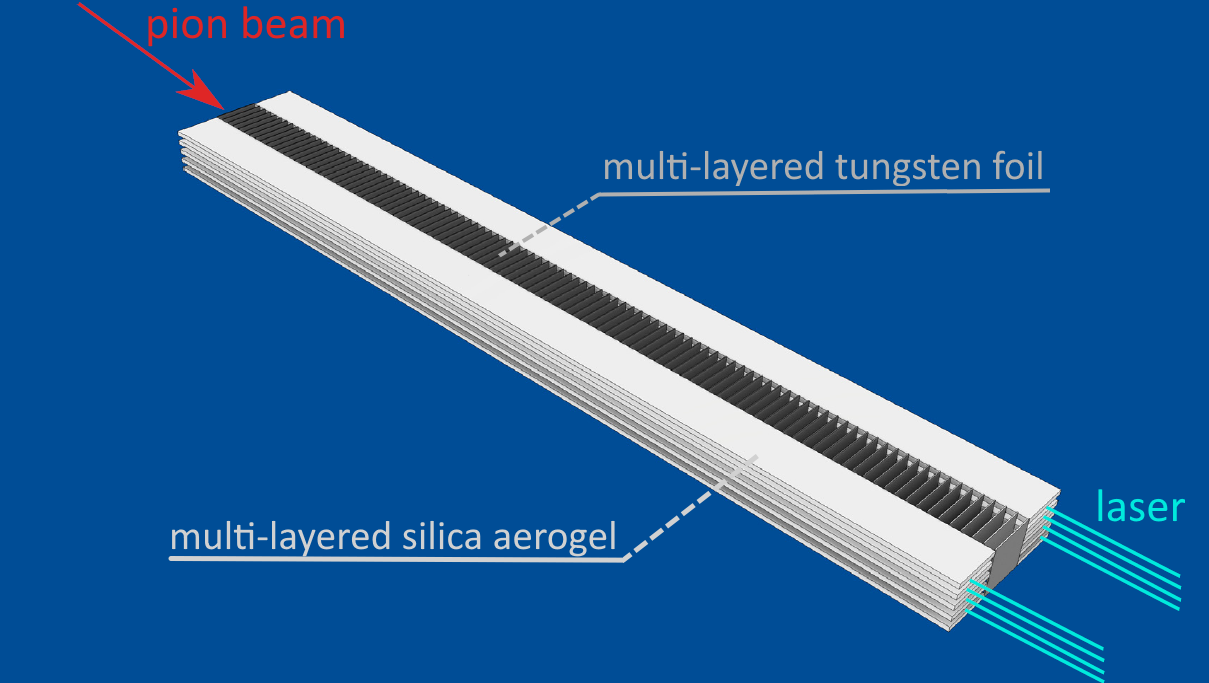
\includegraphics[width=.72\textwidth]{muTRISTAN_muon-production.png}
\caption{The pion stopping target surrounded by silica aerogel for muonium production and laser ionization, as proposed in the $\mu$TRISTAN.\label{fig:multilayer}}
\end{figure}

Muons produced by pion decays then enter a multi-layered silica aerogel structure, where they undergo muonium formation followed by laser ionization to produce the ultra-cold muon beam. \textcolor{blue}{The design and the breakdown efficiency of the multi-layer target design can be found in Ref~\cite{Zhang:2022ilj}. The net efficiency of this critical stage is determined by several sequential processes. The muonium formation probability is about 52\%, as measured in dedicated experiments at TRIUMF using silica aerogel targets, reflecting the intrinsic material properties governing muonium emission~\cite{Bakule:2013poa, Beer:2014ooa}. The vacuum yield of muonium is estimated to be about 60\%, corresponding to the fraction of muonium atoms diffusing out of the aerogel into vacuum; this value is obtained from diffusion-model studies constrained by experimental data and already incorporates the enhancement from the multi-layer aerogel design~\cite{Zhang:2022ilj}. If a single proton bunch configuration were used instead of the current double-bunch scheme, the yield could increase by roughly 30\%, corresponding to an effective value of about 0.78. The survival probability against muon decay is currently about 60\%, primarily determined by the laser illumination window ($\sim$1.8 µs). A shorter timing window of about 0.8 µs, achievable in a single-bunch configuration, would reduce decay losses and increase the survival fraction to roughly $\sim$70\% given the 2.2 µs muon lifetime. Finally, the laser ionization efficiency is assumed to be 73\%, corresponding to the baseline parameters adopted for the J-PARC muon $g\!-\!2$ design (122 nm wavelength with 100 $\mu$J pulse energy)~\cite{Abe:2019thb}; in principle, higher laser power could increase this efficiency to above 80\%~\cite{Zhang:2022ilj}. Combining these factors yields an overall ultra-cold muon production efficiency of $\sim14\%$ for this 10-meter region.}

The ultra-cold muons generated across the 10-meter production zone are longitudinally spread and subsequently collected and focused onto a secondary aerogel target to compress the beam and ensure uniform energy. In this stage, muonium is re-formed and re-ionized by the laser with an assumed efficiency of $50\%$. Consequently, the net efficiency to convert a stopped pion into a usable ultra-cold muon is \textcolor{blue}{$\approx 6.8\%$. The two bunches of muons from the pion production ring are combined at the second muon target by tuning the timing of the laser irradiation. }

Built upon the J-PARC proton accelerator–like facility, the $\mu$TRISTAN proposal suggests a transformative upgrade to meet the high-intensity requirements of a collider. Unlike the J-PARC configuration, where protons strike a target only once, $\mu$TRISTAN introduces a pion production ring. To maximize the yield, the proton beam is directed into a dedicated ring containing a 10-mm-thick graphite target, where the beam is recirculated to strike the target 40 times per bunch. During the hadronic collision, the pion production cross-section is approximately 150 mb at this energy (3 GeV proton beam) regime. Given this target thickness and cross-section, the probability of pion generation is calculated to be $0.016$ pions per incident proton. This recirculation process generates a pions for each turn, resulting in a total of 40 muon bunches per cycle. An integrated RF cavity compensates for the protons' energy loss in every passage through the target.

By multiplying the probabilities of each independent stage, we determine the number of final ultra-cold muons produced per single incident proton:
\textcolor{red}{
$$ \text{Yield} = 0.016 \times 0.50 \times 0.068 = 5.5 \times 10^{-4} \, \mu^+/\text{proton} $$
}
To determine the absolute number of muons generated per second (the instantaneous flux), we integrate this yield over the full macro-pulse structure of the proton driver. When the significant gain in muon collection efficiency is combined with the 40-bunch structure and an upgraded 50 Hz repetition rate, the total instantaneous flux is calculated as:

\textcolor{red}{
$$ \Phi_{\mu} = \left(5.5 \times 10^{-4}\right) \times \left(4.1 \times 10^{13}\right) \times 2 \times 40 \times 50 \approx 9 \times 10^{13} \, \mu^+/\text{s} $$
}
This high-flux, ultra-cold $\mu^+$ source provides the necessary foundation to reach the luminosity goals of the LH$\mu$C.

\textcolor{red}{
Prior to injection into the ERL assumed in the LH$\mu$C design, it is necessary to pre-accelerate the ultra-cold muon beam up to an energy of approximately 500 MeV, corresponding to $\beta \sim 0.98$. This requirement arises from the phase-slip constraint in radio-frequency (RF) accelerating structures optimized for ultra-relativistic particles, as well as from beam-dynamical considerations. Since the electron linac is designed for $\beta \sim 1$, injecting lower-energy muons would lead to significant phase slippage, resulting in a strong reduction of the effective accelerating gradient and eventually making efficient acceleration impractical. Therefore, pre-acceleration to the sub-GeV scale is essential to ensure efficient capture and stable beam transport in the downstream linac. 
}
\par
\textcolor{red}{
While the optimal RF frequency of the pre-acceleration section may be adjusted to match the frequency of the downstream electron linac foreseen in the LH$\mu$C, such a front-end can in principle be realized using a scheme similar to the muon linac currently under development at J-PARC~\cite{Otani:22:PTEP}. This system employs a sequence of low- to intermediate-$\beta$ accelerating structures, enabling efficient acceleration of muons from the initial ultra-cold state to the relativistic regime.
}
\par
\textcolor{red}{
The J-PARC muon linac provides a practical reference for such a pre-acceleration stage, employing a staged configuration optimized over a wide velocity range. Muons are first accelerated and bunched by a 324 MHz RFQ to the sub-MeV scale~\cite{Kondo:15:IPAC}, followed by a 324 MHz IH-DTL for efficient low-$\beta$ acceleration~\cite{Nakazawa:22:PRAB}, after which higher-frequency structures such as an L-band DAW~\cite{Otani:19:JPCS} and an S-band disk-loaded structure (DLS)~\cite{Sumi:23:JPCS} are used to reach the $\sim$200 MeV scale. Up to the IH-DTL stage, actual accelerator components have been constructed and the facility is currently under development toward beam acceleration, while for the downstream sections, proof-of-principle has been demonstrated through prototype cavities. Based on these achievements, further design efforts are underway to realize a more compact and efficient linac extending the energy up to $\sim$500 MeV. This staged approach ensures continuous velocity matching, suppresses phase slippage, and enables rapid acceleration such that muon decay losses remain at an acceptable level (of 20\% or below), making it a realistic basis for the front-end acceleration required in the LH$\mu$C design.
}

\subsubsection{Hybrid \texorpdfstring{$\mu^+$}{muon}-source [Chris]}

\subsubsection{\texorpdfstring{$\mu^+$}{Muon} booster}

vFFA~\cite{max} vs. RCS~\cite{InternationalMuonCollider:2025sys} 


The rapid acceleration of muons from the ultra-cold source to the collision energy of 500~GeV is one of the most critical challenges of the \lhuc design. For acceleration technology, the Muon Collider baseline currently favors a Hybrid Rapid Cycling Synchrotron (Hybrid-RCS) \cite{taylor2025mucol}. This approach interleaves fixed-field superconducting magnets with fast-ramping normal conducting ones to accelerate a single bunch \cite{black2024muon}. Hybrid-RCS utilizes fast-ramping dipoles to maintain a fixed circular orbit during acceleration. While the underlying beam dynamics are well-understood, the required ramping rates pose severe technological challenges regarding power consumption, power supply synchronization, and eddy current losses in the magnets.

 

To circumvent the fundamental limitations of fast-ramping magnetic fields inherent in RCS designs, a novel acceleration scheme based on the Fixed-Field Alternating Gradient (FFAG) principle is proposed. First conceptualized in the 1950s, the FFAG architecture combines the continuous-wave (CW) beam capability of a cyclotron with the strong-focusing properties of a synchrotron. Because the magnetic fields in an FFAG remain completely static (constant in time), it entirely eliminates the issues of eddy currents, complex power supply synchronization, and inductive power losses. This static nature is exceptionally well-suited for the rapid acceleration required by short-lived muons.

Traditional FFAGs, however, accommodate the increasing momentum of the particle beam through a horizontal excursion (hFFA), meaning the beam spirals radially outward as it gains energy. For a multi-TeV energy range, this horizontal spread dictates unacceptably wide and heavy magnets, making hFFAs economically and practically unfeasible for a high-energy muon acceleration.

For this purpose, the \lhuc booster design is based on the vertical excursion Fixed-Field Accelerator (vFFA). In a vFFA, the bending magnetic field is designed to increase exponentially along the vertical axis, described by $B(y) = B_0 e^{ky}$, where $k$ is the field index. As the muons are accelerated, their orbit does not expand radially; instead, the entire beam shifts vertically upwards into regions of stronger magnetic field. This vertical climbing mechanism provides the necessary bending rigidity for higher-energy particles while keeping the footprint of the accelerator strictly isochronous and remarkably compact in the radial plane.

However, accommodating a massive momentum spread (from a few hundred MeV to 500~GeV muon energy) within a single, continuous vFFA arc poses insurmountable engineering challenges. In the exponential field profile, the ratio of the final to initial momentum ($p_{max}/p_{min}$) is directly proportional to $e^{k \Delta y}$. If a single arc were utilized for the entire hundreds of MeV to 500~GeV range, it would demand either an unrealistically large $\Delta y$ or an extreme $k$ index. A massive vertical aperture implies manufacturing extremely tall superconducting magnets with massive cryostats, leading to exorbitant costs and severe mechanical instabilities. Conversely, pushing the $k$ index to extreme values results in highly non-linear and unmanageable magnetic fringe fields, destroying the dynamic aperture and causing immediate beam loss.

To resolve this technological deadlock, a pragmatic and highly cost-effective strategy is proposed: maximizing the synergy with the proposed LHeC infrastructure. Instead of designing a massive, all-encompassing vFFA from scratch, the \lhuc booster adopts a smartly integrated 3-stage cascading architecture like LHeC has. The fundamental design criterion for this cascade is to limit the momentum ratio ($p_{max}/p_{min}$) in each dedicated vFFA stage to a factor of approximately 4. This specific ratio elegantly balances the $k$ index and the required $\Delta y$, keeping magnet manufacturing well within current engineering limits and ensuring optical stability. For the \lhuc booster cascades, a unified field index of $k=15~m^{-1}$ has been selected to optimally balance these constraints without introducing severe fringe-field non-linearities. 

The facility is constrained by the geometry of the proposed LHeC tunnel, which features a racetrack shape with two 1.5 km straight sections and two 1 km radius arc tunnels designed to host cascaded arcs. The 3-stage acceleration sequence is structured as follows:

\begin{itemize}

    \item \textbf{STAGE 1 (first acceleration stage utilizing LHeC arc infrastructure):} To minimize costs and maximize muon survival, the initial acceleration from 0.5~GeV up to 36.5~GeV utilizes the existing LHeC linear accelerators and stage-one fixed-field arcs. Crucially, the beam executes exactly 1.5 turns, passing through the 12~GeV linacs three times in total, and is sequentially routed into the corresponding energy-matched arcs for a strict single pass. This 1.5-turn routing rapidly boosts muons to relativistic speeds, eliminating the need for dedicated, complex low-energy vFFA or RCS rings.

    In case the three-pass ERL is available, the muon beam passes linacs 7 times reaching the energy after stage one of 87.5~GeV.
    
    \item \textbf{STAGE 2 (first vFFA stage):} Once the muons reach 36.5~GeV, they are injected into the first dedicated vFFA ring. This stage accelerates the beam from 36.5~GeV to 144.5~GeV. By keeping the energy ratio at 3.96 ($=144.5/36.5$), the required vertical aperture and $k$ index remain highly manageable, avoiding extreme magnet dimensions and allowing for an average magnetic field of merely $\approx 0.4$~T. With $k=15$~m$^{-1}$, the required vertical beam excursion is $\Delta y = \ln(4.0) / 15~m^{-1} \approx 9.2~cm$.
 
    \item \textbf{STAGE 3 (second high-energy vFFA stage):} Upon the intermediate stage at 144.5~GeV the beam enters the final vFFA arc. This final acceleration phase takes the beam to the 504.5~GeV beam energy. With an energy ratio of roughly 3.5 ($=504.5/144.5$), this main vFFA ring operates optimally without pushing the boundaries of NbTi superconducting limits or requiring unfeasible vertical apertures. Using the same field index, the vertical excursion is reduced to $\Delta y = \ln(3.85) / 15~\text{m}^{-1} \approx 9.0~cm$.

    In the 80~GeV case at stage one acceleration, perhaps only one vFFA stage will be sufficient.
\end{itemize}

To safely accommodate $\Delta y <10$~cm vertical climb along with operational margins and horizontal orbit scalloping, the \lhuc vFFA magnets could be designed with a full aperture of 15~cm.

In modern accelerator design, pushing magnetic fields beyond 8~T requires advanced, brittle, and expensive superconducting materials like Nb$_3$Sn or High-Temperature Superconductors (HTS), which severely complicate the winding of 3D Canted-Cosine-Theta (CCT) vFFA coils. Conversely, enforcing a strict 8~T upper bound allows the exclusive use of reliable, cost-effective NbTi technology, the proven workhorse of modern accelerators. Consequently, this 8~T limit serves as a fundamental design constraint for the \lhuc booster ring.

To adhere strictly to this limit while maintaining perfect optical stability, both ARC 2 and ARC 3 utilize a symmetric D-F-D (Defocusing-Focusing-Defocusing) triplet cell. Lattice optimization focuses exclusively on the ultimate bottleneck: ARC 3 at its 500~GeV peak ($y \approx 9.6$~cm). For a 1~km radius tunnel, the required average field ($B_{avg}$) at 500~GeV is merely $\approx 1.67$~T. However, the vFFA's alternating gradient demands immense, opposing local fields.

Numerical optimizations for this 500~GeV peak yield an effective optical length of 6~m for the central focusing ($F$) magnet, a combined length of 3~m for the defocusing ($D$) element, and 2~m of total drift space, resulting in an exact 11~m cell footprint. To conform to the 1~km radius LHeC racetrack arcs, this geometry dictates a precise topological requirement of 286 consecutive cells per arc, totaling 572 cells for the complete high-energy stage. At the operational maximum, this distributed layout keeps the focusing field well within safe margins at $B_{Fpeak} \approx 5.5$~T, and the defocusing field at $B_{Dpeak} \approx -4.9$~T. By peaking comfortably below the hardware threshold, the \lhuc design preserves the dynamic aperture and effectively minimizes quench risks.

\subsubsection{\texorpdfstring{$\mu^+$}{Muon} main ring}

The 500 GeV muon beam emerging from the booster ring, the final stage of the accelerator chain, is transferred to the circular main ring positioned tangentially to the LHC tunnel. The physical bending radius required to keep the muons in orbit within this ring is determined by the relationship between momentum and magnetic field strength, $B\rho \approx 3.335 \cdot p$. Utilizing standard 8.3 T superconducting LHC dipole magnets, the bending radius for 500 GeV muons is calculated to be approximately 0.2 km. This radius dictates that the total length of the magnetic arcs, where solely the bending occurs, is approximately 1.3 km.

Beyond the bending magnets, the geometry of the main ring is designed to accommodate the straight sections essential for beam dynamics and collision physics. In this context, the ring structure incorporates an approximately 150-meter main Interaction Point (IP) region to house a large-scale general-purpose detector and its low-$\beta$ focusing quadrupoles, an approximately 50-meter injection region to bring the beam into orbit, and approximately 300 meters of operational space distributed throughout the ring for focusing quadrupoles and other orbit corrector systems. In this design, which negates the need for RF cavities due to the short lifetime of muons and their negligible synchrotron radiation, the addition of all these components brings the total circumference of the ring to approximately 1.8 km.

The short half-life of muons is the primary physical motivation behind this 1.8-kilometer design. When a muon, with a rest mass of 105.6 MeV, reaches an energy of 500 GeV, its Lorentz factor increases to $\gamma \approx 4735$, and according to special relativity, its lifetime in the laboratory frame extends to $\tau = \gamma \tau_0 \approx 10.4\text{ ms}$. Traveling close to the speed of light, these particles can cover a total distance of approximately 3120 km before their beam intensity drops to a $1/e$ ratio. In this main ring with a total circumference of 1.8 km, the muons can complete approximately 1750 turns in orbit before decaying. Since luminosity ($L$) in muon colliders is inversely proportional to the ring circumference ($L \propto 1/C$), maintaining the circumference in the 1.8 km range with 8.3 T magnets minimizes the decay losses per turn, thereby maximizing the collision frequency achieved over these 1750 turns.

Due to the hybrid nature of the LH$\mu$C project, the muon beam in the main ring must be perfectly synchronized with the proton beams in the LHC at the interaction point. Considering the standard 25 ns bunch spacing structure of the LHC, the timing of the 40 muon bunches to be injected into the main ring must be adjusted to be a multiple of this frequency. Since the main ring lacks RF systems to control the bunch structure, the required bunch spacing and phase matching with the protons are fixed during the booster ring stage, immediately before the muons are injected into the 1.8-kilometer main ring. This precise synchronization ensures that every time the muons circulating the ring pass through the interaction point, they collide exactly on time with the corresponding oncoming proton bunch.


\subsubsection{Proton ring performance}

increasing the proton bunch charge at lower collisions rate

\subsubsection{Interaction region/MDI}

There are two options to consider for the focusing of muon beam:
\begin{itemize}
    \item to make focusing of muons close to the IP, "in between" the mini beta quadrupoles of the LHC, as is proposed for electrons at the LHeC;
    \item to make focusing of muons "oustside" mini beta quadrupoles of the LHC,
in a "linear collider type style".
\end{itemize}

The time separation of muon bunches is large at \lhuc, of 300~ns nominally, corresponding to the first "passing by" of the proton and muon bunches at 45~m from the IP. Therefore, a very small crossing angle, $\ll 100~\mu$rad is needed to avoid parasitic collisions of muon and proton bunches. 

To achieve a "mechanical" separation of the muon and proton beams, the most preferred scheme is by introducing a new
separator dipole, which in combination with the LHC D1 \& D2 dipoles would create a closed 3-bump, allowing to restore the LHC design orbit after D2.

Of course, the effects of "muon magnets" 
on the proton beam remain to be checked,
perhaps requiring a compensation scheme.
In addition, a full muon optics needs to be established, including the feasibility of the muon magnets.

Last but not least, the appropriate shielding of the beam-lines against the background due to the beam muon decays has to be studied and properly designed. 

\subsubsection{1 and 2 TeV upgrades}

First, the main ring must then have a circumference of about 3.3(6.3)~km for the 1(2) TeV case.

Then, to reach the muon beam energy of 1 TeV, while maintaining the muon beam high intensity at the top energy, we assume upgrading the linac's acceleration to 15~GeV. It can be achieved by making it longer or/and by increasing the acceleration gradient. For example, an extension of the linac lengths by 250~m for the 23 MeV/m gradient of the RF cavities results in an acceleration of 30~GeV per turn. A combination of a one pass ERL (to reach 45~GeV) and a 2-stage vFFA booster may be used.

Reaching the maximum energy of 2~TeV might require an extension of the linac lengths by 500(750)~m for the 29(23)~MeV/m gradient of the RF cavities, to obtain a 40~GeV acceleration per turn. 

\subsubsection{\texorpdfstring{LH$\mu$C}{LHuC} performance}

The physics reach of the proposed LH$\mu$C is fundamentally governed by its deliverable luminosity. Unlike stable proton or electron beams, the short lifetime of the muon renders the bunch intensity a time-dependent variable, requiring a rigorous dynamic approach to evaluate the overall collision performance. As the beam circulates the main ring, the muon population in a given bunch is observed to decrease from an initial $7.2 \times 10^9$ muons down to an effective average of $4.5 \times 10^9$ muons over the duration of the store.

Considering the initial muon bunch intensity exiting the booster ring, the precise calculation of the muon population reduction and the subsequent luminosity evolution within the main ring was assigned to the AloHEP (A luminosity optimizer for High Energy Physics) software [?]. AloHEP is a dedicated software tool developed for collider simulation, focusing on comprehensive beam dynamics calculations at the interaction region. It computes crucial collision parameters (such as luminosity, beam-beam tune shift, and disruption parameters) for various collider architectures (linear, circular, linac-ring) and diverse particle beams (electrons, positrons, muons, protons, nuclei). By utilizing the geometric and magnetic parameters of the main ring, AloHEP accurately simulates the interaction region, rigorously accounting for significant luminosity-altering phenomena, including the pinch effect, the hourglass effect, and particle decay.


\begin{table}[htbp]
\centering
\caption{Main parameters of the $\mu^+$ beam.}
\label{tab:muon_params}
\begin{tabular}{lcc}
\hline
\textbf{Parameter} &  \textbf{Value} \\
\hline
Muons per bunch [$10^9$] & 7.2 \\
Beam energy [GeV] & 500 \\
$\beta_{x,y}$ @ IP [cm] & 2.5 \\
Bunch length [mm] & 2 \\
Transverse $\varepsilon_{x,y}$ [nm] & 0.75 \\
Bunches per ring & 40 \\
Bunch spacing [ns] & 250 \\
Circumference [km] & 1.8 \\
\hline
\end{tabular}
\end{table}

The main parameters of the antimuon beam utilized in these simulations are presented in Table \ref{tab:muon_params}. The initial numbers of antimuons are determined by the population exiting the booster ring, as discussed in the preceding subsection. To maintain consistency with the finalized circular main ring design, the beam energy is set to 500 GeV, and the circumference is 1.8 km. Consequently, with 40 bunches circulating 1750 times in the ring and repetition rate 50 Hz, the collision frequency is adjusted to 3.5 MHz. Let us mention that $\beta_{x,y} = 2.8$ cm is chosen for matching with transverse size of the LHC proton beam at the interaction point.

For the proton beam, the parameters utilized for the luminosity calculations in the LH$\mu$C are adopted from the proton beam parameters for LH$e$C project [LHeC CDR], assuming four times larger bunch charges, which are presented in Table \ref{tab:proton_params}.

\begin{table}[htbp]
\centering
\caption{Proton beam parameters.}
\label{tab:proton_params}
\begin{tabular}{lc}
\hline
\textbf{Parameter} & \textbf{Value} \\
\hline
Protons per Bunch [$10^{11}$] & 4.4 \\
Beam Energy [TeV] & 7 \\
$\beta_{x,y}$ @ IP [cm] & 7 \\
Transverse $\varepsilon_{x,y}$ [nm] & 0.33 \\
Bunch spacing [ns] & 250 \\
\hline
\end{tabular}
\end{table}

Using the antimuon and proton parameters defined Table  \ref{tab:muon_params} and Table  \ref{tab:proton_params}, the luminosity value is calculated within the AloHEP software. The resulting main parameters of the LH$\mu$C collider are summarized in Table \ref{tab:final_performance}.

\begin{table}[htbp]
\centering
\caption{Main parameters of the LH$\mu$C collider.}
\label{tab:final_performance}
\begin{tabular}{lcc}
\hline
\textbf{Parameter} & \multicolumn{2}{c}{\textbf{Value}} \\
\hline
Center-of-mass energy, $\sqrt{s}$ [TeV] & \multicolumn{2}{c}{3.74} \\
Peak(?) luminosity, $\mathcal{L}$ [$10^{33} \text{ cm}^{-2}\text{s}^{-1}$] & \multicolumn{2}{c}{4.3} \\
\hline
\textbf{Beam parameters} & $\mu^+$ & $p$ \\
\hline
RMS beam size at IP, $\sigma_{x,y}$ [$\mu$m] & 4.8 & 4.8 \\
Beam-beam parameter, $\xi_{x,y}$ [$10^{-4}$] & 600 & 3.5 \\
\hline
\end{tabular}
\end{table}

Muon beam polarization...

Discussion of the \lhuc energy consumption...

\subsubsection{Neutrino flux}

\subsubsection{HE-LH$\mu$C and FCC-$\mu$h cases}

Building on the \lhuc experience,
a 5 TeV muon beam at the FCC-hh would provide high-luminosity $\mu p$ collisions at $\sqrt{s}=30$~TeV.
For the physics case, the data sample of 10~ab$^{-1}$ and polarization of 70\% is assumed.

In the same manner, a 4 TeV muon beam at the HE-LHC would provide high-luminosity $\mu p$ collisions at $\sqrt{s}=15$~TeV.
For the physics case, the data sample of 5~ab$^{-1}$ and polarization of 70\% is assumed.

\subsubsection{Outlook/next steps}

\newpage

\section{Detectors [Ilhan, Laurent]}
\label{sec:detectors}

In this white paper, all technologies assumed in the definition of the detectors design are chosen through their maturity for integration.
Thus, none of the sub-detectors proposed require a major R\&D effort threatening the implementation of the LHeC/\lhuc detector concepts discussed here.

\subsection{LHeC}
\label{subsec:detLHeC}

\subsubsection{Flagship design: 50--60 GeV electron beams}

The main design choices for the LHeC detector concept are described in \cite{LHeCStudyGroup:2012zhm,LHeC:2020van,Ahmadova:2025vzd}.
From the interaction region outwards, and as depicted in Fig.\,\ref{fig:lhec_detector_concept}, a longitudinally asymmetric tracker surrounds the interaction point.
It relies on existing CMOS technologies, with a central barrel composed of 4 layers of pixels and 5 layers of macro-pixels, 2 wheels in the central endcaps, and 3 and 5 wheels in the backward (following the electron direction), and forward (hadron direction) endcaps respectively.

Consecutive to the tracker component, both a barrel and end caps section of an electromagnetic, and a hadronic calorimeters are located outside the volume of an inner superconducting 3.5~T solenoid.
For the barrel section, the proposed design for the electromagnetic part is a liquid argon calorimeter ($28-30X_0$) with an ATLAS-like accordion structure, and a hadronic part composed of iron absorbers adding up to an interaction length $\sim8-12\lambda_I$.

Finally, at the outermost section of the LHeC detector, an array of muon detectors is placed with gas chambers technologies already successfully operating in the (HL-)LHC environment: resistive plate chambers, cathode strip chambers, and others.

\begin{figure}
\centering
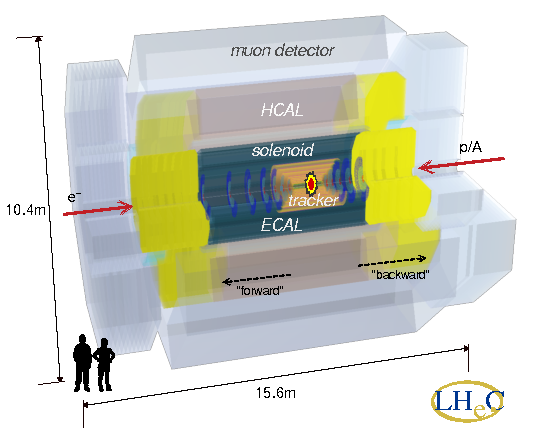
\includegraphics[width=.8\textwidth]{lhec_detector_annotated_nobackground.pdf}
\caption{Cutaway drawing of the LHeC detector concept as described in the CDR, and bridge concept papers.}
\label{fig:lhec_detector_concept}
\end{figure}

\add{[synchrotron radiation study]}

Outside the interaction region, a circular-elliptic geometry for the beamline is optimised to fit the dynamics of a three-beam system.
Furthermore, it allows an efficient fanning of the synchrotron radiation emitted by the lepton bending close to the interaction point.

While a detailed simulation of all detector components described in this section is required for the optimisation of key operational parameters, this goes beyond the scope of this proposal.
Both a DELPHES 3 detector description of all appartuses, and a Key4hep stack are however under construction, and will be described in a follow-up publication.

\subsubsection{Staged design: 20 GeV electron beams}

In the case of a staged configuration as described in \cite{Andre:2025iar}, a lower energy baseline may be defined as a first step in the construction of the nominal LHeC.
Based on a single-pass acceleration through the two 10-GeV linacs, the 20 GeV electron beam configuration induces an additional boost of the central system in the direction of the proton.
Therefore, a modified design covering an extended rapidity acceptance is required to ensure a good reconstruction of flagship DIS, $t\bar t$, and Higgs final states.
This includes calorimetry up to $\eta\sim$ \add{xxx}, and good tracking performances at a shorter distance to the beams, thus in a challenging radiation environment, especially in the very forward region.

The centre-of-mass energy for electron-hadron being reduced from $1.2$ to $0.75$ TeV in this operational mode, the radiative power emitted mainly by synchrotron radiation, is also reduced by a factor \add{XXX}, thus diminishing the need for additional shielding of the critical proton focussing/defocussing quadrupoles in the vicinity of the electron bending magnets.
This allows a relaxed design of the very forward region of the detector acceptance, and the possibility of an increased segmentation in this region of interest.

\subsubsection{Forward proton detectors}

Specific physics cases (e.g. involving the exchange of a colour-singlet such as photons, or pomerons, \ldots) allow high-energy interactions to occur in the vicinity of the lepton-hadron collision point without the fragmentation of the scattered proton after the exchange.
Referred to as central exclusive processes (CEP), these provide a laboratory for low-rate, high-precision searches described in section \ref{paragraph:twophoton}.
Instrumentation of the forward near-beam region is crucial for the direct tagging of this particular class of events where a proton is detected, and to precisely determine the scattered muons momentum to ensure a good reconstruction of the the DIS kinematic variables.
Multiple technologies have already demonstrated their ability to observe the scattered protons a few units of the beam separation $\sigma_{x,y}$ in a radiation-hard environment: so-called Roman Pots \cite{CMS:2024xbs,ATLAS:2024ztz}, or moveable (Hamburg) beam pipes.
Both the proton, and the lepton spectrometer systems may therefore consist of heterogeneous detectors composed of layers of silicon-based tracking detectors, such as the ones of the CMS Precision Proton Spectrometer \cite{CMS:2014sdw} and its HL-LHC upgrade \cite{CMS:2021ncv}.

%in the far forward direction and a muon system in the far backward direction mounted on the beam pipe outside the detector able to measure muons with reasonable resolution down to very small scattering angles and at momenta up to the beam to detect the scattered protons and muons, respectively.


\subsection{\texorpdfstring{LH$\mu$C}{LHuC}}
\label{subsec:detLHuC}

Recently, general-purpose detector design studies have been presented for the detection of particles produced by muon-hadron collisions\cite{Acosta:2023,Akturk:2025ubm}. The detector structure given in these studies is configured superconducting solenoid magnet for precise momentum measurements for charged tracks. It consists of a silicon tracker to provide precision timing and position information, a particle identification system located outside of the silicon tracker, electromagnetic and hadronic calorimeters to precisely measure the energies of the particles, and muon spectrometer to measure muons with proper resolution. These sub-detectors surround the beam pipe. On the beam pipe outside the detector, Roman Pots in the far forward direction and a Muon System in the far backward direction are mounted to detect the scattered protons and muons, respectively. 

Beam induced backgrounds are one of the main challenges in designing the muon collider detectors. The case for muon-hadron collision requires the consideration of shielding of critical elements following the direction of the muon beam. This latter, with a flux estimated at high values in the design luminosity considered here, is expected to deliver an intense source of secondary radiation through ionisation and bremsstrahlung emissions. In order to protect the innermost detector elements, a tungsten nozzle shielding cladded with borated polyethylene is placed on the coming muon side.

The studies on dedicated detector design will be performed corresponding to the acceptance, resolution, and calibration goals which arise from the muon-hadron collision physics programs. The realistic dimensions of the detector and its sub-components will be determined using detailed GEANT4 and FLUKA simulations to get the detector's response to particles generated from the collision. Shielding studies will be detailed to optimize the overall physical performance of the detector. The variations of the energy depositions at different muon energies traversing such a cone made of different stopping target materials will be studied. 


\subsubsection{Physics motivated requirements}

In order to translate the kinematic requirements defined for the LHeC/\lhuc physics case described in Section\,\ref{sec:physics} into constraints on acceptance and rates estimates, a {DELPHES} 3 \cite{deFavereau:2013fsa} modeling of the detector concept is defined. During modeling, the physical requirements mentioned below should also be considered based on the geometry defined for the LHeC CDR studies.


As the baseline \lhuc described here proposes the collision of a 7 TeV proton beam against a 1 TeV muon beam, the instrumentation of the detector is asymmetric, following the asymmetric nature of the collisions.
The physics program of the muon-hadron collision motivates strict demands for detector such as hermetic coverage, strong forward and backward acceptance, precision tracking, a finely segmented calorimetry system, and a good shielding from beam induced background. 

Following the physics case described in Section \ref{sec:physics}, the production of BSM particle decaying to missing energy final states imposes detector hermeticity for missing energy signatures.
In terms of the DIS kinematics, the proton structure is precisely examined over an extended Bjorken-x and $Q^2$ phase space. This strongly motivates excellent forward and backward acceptance, precise measurement of the small-angle scattered lepton and hadronic final state.

A major source of the beam induced background is the decay of primary muons and the interaction of their decay products with the beam pipe.
In order to prevent the decay products from entering the detector, the muon beam line should be coated with a tungsten nozzle. The nozzle is coated with borated polyethylene to reduce the amount of neutrons produced from interactions within the tungsten core. The occupancy in the tracking system could be improved with the optimized nozzle.

For the precision of the electroweak and QCD measurements, high-resolution central tracking and finely segmented electromagnetic calorimetry should be used. A silicon tracker system with precision timing information is critical for performing meaningful physics analyzes. It would have 4-D tracking using Low Gain Avalanche Diodes (LGADs) or  PICOSEC-Micromegas (PICOSEC-MM) \cite{Malberti:2026}. The particle identification system is crucial for QCD measurements. Maintaining a very high tracker occupancy under beam-induced background conditions is an essential performance factor.

\subsubsection{\texorpdfstring{$\mu^+$}{Muon} shielding}

With a fraction of the muons decaying despite their acceleration in the relativistic regime, a large amount of background particles such as photons, electrons and neutrons are expected in the vicinity of the interaction region.
These particles are foreseen to generate visible signals in the detector, undistinguishable from the muon-hadron collisions.
The effect of beam-induced background depends on the energy of the muon beam, machine optics, and lattice elements.
According to previous studies~\cite{Collamati:2021,Bell:2025}, massive reductions of beam induced backgrounds can be obtained by means of a careful optimization of the Machine Detector Interface (MDI) and timing selection.
A conical tungsten nozzle cladded with borated polyethylene, placed around the muon beam line near the interaction point, is also used as the primary beam induced backgrounds mitigation element.
Its main purpose is to block the muon decay products before they enter the sensitive detector volume. 

After the collision, the scattered partons (e.g., jets) and muons are mostly going towards the backward (proton coming side) direction. The presence of the nozzle in the backward region is considered undesirable from the perspective of precision muon measurements.
Studies have shown that the passage of high-energy muons through a thick tungsten cone leads to non-negligible energy loss and multiple Coulomb scattering.
For a 1 TeV muon traversing a 6 m tungsten nozzle placed in the backward region, these effects generate a significant low-energy tail and angular smearing in the outgoing muon, which in turn degrades the resolution of reconstructed kinematic observables such as Q\textsuperscript{2}. Thus, shielding tungsten nozzle is applied only to the muon coming side \cite{Acosta:2023,Akturk:2025ubm}.

However, the nozzle placed in the forward region affects the physical performance by limiting the angular acceptance of the detector.
Therefore a careful optimization of this component is required to increase the detector angular acceptance while lowering material costs.
This study is carried out to minimize beam-induced background noise and the total volume of the nozzle.
One may cite the previous work performed for the shielding optimization at Muon Collider using FLUKA simulation by varying three key geometrical parameters: the angle of the nozzle tip, $\Theta_{\rm nozzle}$, the position along the beam axis where the aperture changes, $z_{\rm change}$, and the base radius, $r_{\rm base}$ \cite{Castelli:2025}.
One may also note that reducing the nozzle size lowers the overall weight that needs to be supported, simplifying the design of the nozzle’s supporting structure and creating more space for detectors, thereby enhancing the angular acceptance of the detector.

\subsubsection{Re-use of/synergy with LHeC detectors}

LHeC is the first lepton hadron collider reaching center of mass collision energies at the TeV range, using the 7 TeV proton beam and an electron beam energy of 60 GeV.
The design of the LHeC detector, with its trackers, calorimeters, and alike was previously described in CDRs, and builds opportunities for the construction of new collider detectors.
The designed detector already includes many of the key features required for high-precision muon-hadron collision physics program, including an hermetic coverage, a strong forward acceptance, and a well-balanced tracking and calorimetry system.
Thus most segments of the baseline LHeC detector can be expected to remain directly applicable with some required modifications for a muon-hadron collider.
Leveraging this completed design provides both technical and cost advantages.

However, the presence of a high-energy muon beam introduces a fundamentally different background environment then the original electron–proton configuration of the LHeC detector.
Without dedicated shielding, beam induced backgrounds would lead to unacceptably high detector occupancies, radiation loads, and trigger rates.
An optimized shielding strategy on the muon side is therefore a main requirement of the muon-hadron collider detector concept.
In order to mitigate the impact of the beam induced background, the nozzle described above should be located inside the LHeC detector in the forward regions along the beam axis from the IP, as seen in Fig.\,\ref{fig:modified_LHeC}.
As the scattered muons are mostly going towards the backward direction, the forward muon part of the detector is removed.
\begin{figure}
\centering
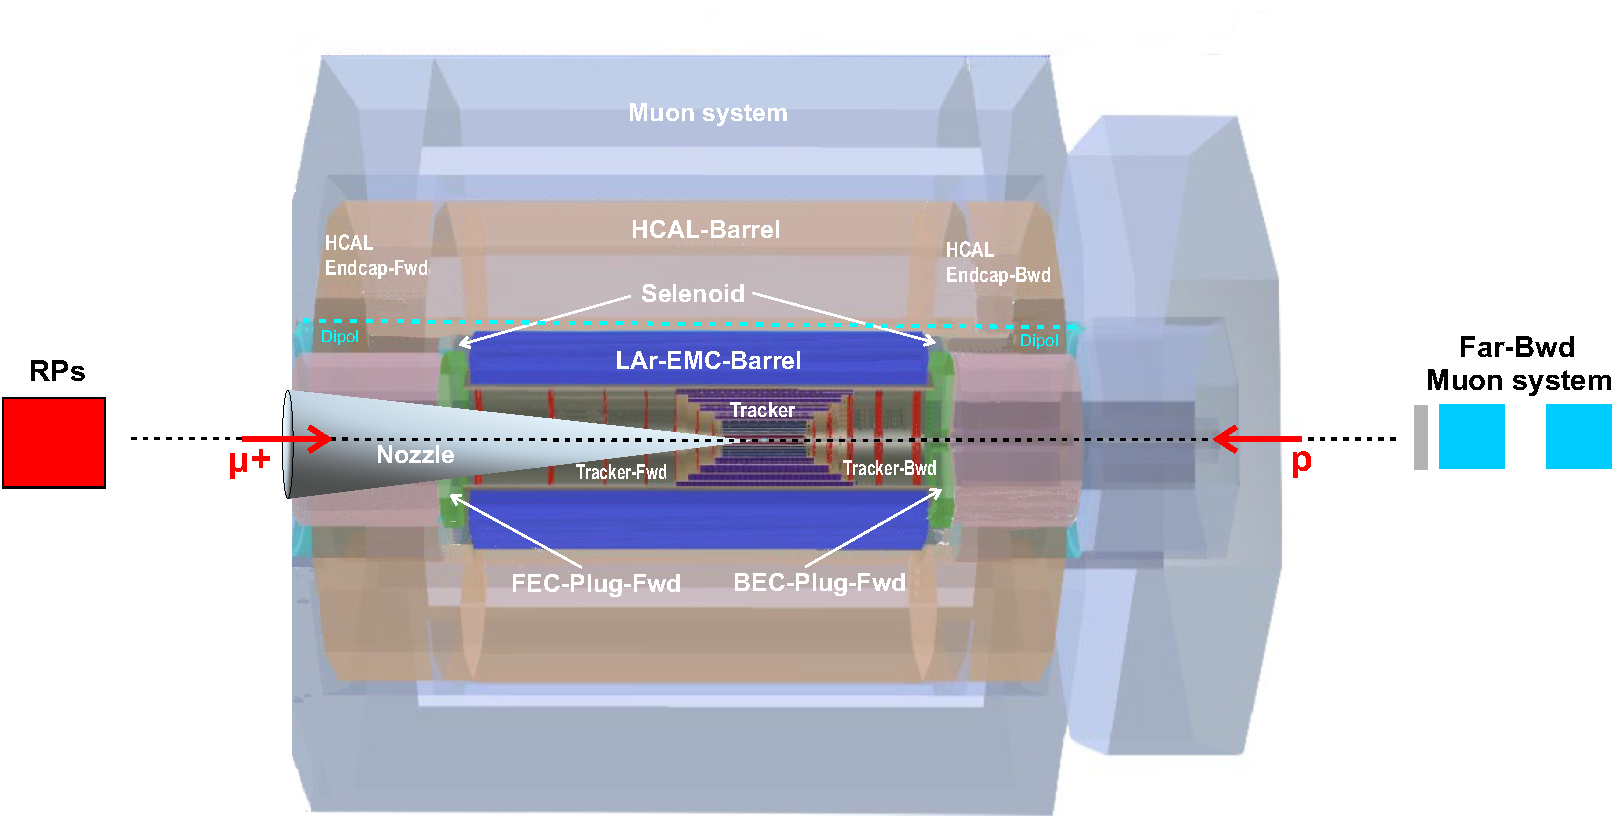
\includegraphics[width=.9\textwidth]{modified_LHeC.pdf}
\caption{Modified LHeC detector for muon-hadron collider.}
\label{fig:modified_LHeC}
\end{figure}

The following changes, such as increased small angle acceptance, background control and mechanical redesign can be implemented preserving the overall LHeC detector architecture.
Small angle physics in the forward direction will be partially lost due to the presence of the nozzle, while the backward acceptance would remain largely preserved. The angle of the nozzle tip should be selected carefully so that it fits well with the beam pipe, final focus magnets, and service lines. Fast timing detectors with precise timing resolution such as LGADs or  PICOSEC-MM should be added to precisely measure the arrival time of particles, allowing the system to distinguish true physics events from delayed background hits. Successful integration requires a joint optimization of the Machine Detector Interface and the timing systems.

\paragraph {\bf Forward Proton Detectors}

While a design and location along the forward beamline suitable for both the LHeC and \lhuc kinematics is preferable in this already highly instrumented region of the accelerator (beam position monitors, beam loss monitors, \ldots), it is subject to a precise study of the beam dynamics in the vicinity of the interaction point, leading to multiple \add{(??)} regions of interest.



\subsubsection{Far Backward Muon Detection}

Additionally, a possibly pre-existing array of Roman Pots in the far forward direction is completed with a Muon System in the far backward direction.
Both are mounted on the beam pipe outside the detector to detect protons and muons with small scattering angles.

With a high-energy incident muon beam, this muon detection in the downstream muon direction (backward) would be essential for DIS measurements and helpful for vector boson fusion processes as well.
Scattering angles can be very small, so detection along the beam line at high pseudorapidity would be required.
For example, DIS scattering with a 1~TeV muon beam leads to muons with $|\eta| \le 7$ for $Q^2\ge  3$~GeV$^2$.
Measuring such TeV muons with a magnet spectrometer is challenging.

One possibility to provide sufficient $\int B\cdot {\rm d}l$ bending is to use the endcap toroid design of the ATLAS experiment \cite{ATLAS:2008xda,ATLAS-Toroid} to instrument several stations along the beamline.
This magnet provides a maximum field of 4.1~T at the innermost radius of 1.05~m (the outer radius is 5.1~m).
Muon detector layers could be placed in front and behind the toroid magnet to measure the bending in the radial direction.
Each magnet could span about 1.6 units of pseudorapidity, so up to 3 stations at ever increasing distance from the collision point would be necessary to fully cover the scattered muon kinematics beyond the central region of the experiment, i.e. $|\eta| \gtrsim 2 $.
This would correspond to stations located roughly 20, 100, and 500~m downstream of the collision point. 

The momentum resolution depends on the precision of the detector technology used. If the achieved detector resolution is of order 150~$\mu$m in front and behind the toroid, then the average momentum resolution (increasing linearly with radius) would be about 5\% at 1~TeV. 

\subsubsection{...}

\subsection{Outlook/next steps}



\newpage

\section{Conclusions [Krzysztof, Saleh]}
\label{sec:conclusions}

great science + huge impact on present and future projects at CERN and worldwide

\newpage

\bibliographystyle{JHEP}
\bibliography{biblio.bib,small-x.bib}



\acknowledgments

This is the most common positions for acknowledgments. A macro is
available to maintain the same layout and spelling of the heading.

\paragraph{Note added.} This is also a good position for notes added
after the paper has been written.


% Bibliography

%% [A] Recommended: using JHEP.bst file
%% \bibliographystyle{JHEP}
%% \bibliography{biblio.bib}

%% or
%% [B] Manual formatting (see below)
%% (i) We suggest to always provide author, title and journal data or doi:
%% in short all the informations that clearly identify a document.
%% (ii) please avoid comments such as "For a review'', "For some examples",
%% "and references therein" or move them in the text. In general, please leave only references in the bibliography and move all
%% accessory text in footnotes.
%% (iii) Also, please have only one work for each \bibitem.

\end{document}
